%% Copyright 2019-2024 Elsevier Ltd
%% 
%% This file is part of the 'CAS Bundle'.
%% --------------------------------------
%% 
%% It may be distributed under the conditions of the LaTeX Project Public
%% License, either version 1.3c of this license or (at your option) any
%% later version.  The latest version of this license is in
%%    http://www.latex-project.org/lppl.txt
%% and version 1.3c or later is part of all distributions of LaTeX
%% version 1999/12/01 or later.
%% 
%% The list of all files belonging to the 'CAS Bundle' is
%% given in the file `manifest.txt'.
%% 
%% Template article for cas-sc documentclass for 
%% double column output.

\documentclass[a4paper,fleqn]{cas-sc}

% If the frontmatter runs over more than one page
% use the longmktitle option.

%\documentclass[a4paper,fleqn,longmktitle]{cas-sc}

%\usepackage[numbers]{natbib}
%\usepackage[authoryear]{natbib}
\usepackage[authoryear,longnamesfirst]{natbib}
\usepackage{tikz}
\usetikzlibrary{arrows.meta,positioning}

%%%Author macros
\def\tsc#1{\csdef{#1}{\textsc{\lowercase{#1}}\xspace}}
\tsc{WGM}
\tsc{QE}
%%%

% Uncomment and use as if needed
%\newtheorem{theorem}{Theorem}
%\newtheorem{lemma}[theorem]{Lemma}
%\newdefinition{rmk}{Remark}
%\newproof{pf}{Proof}
%\newproof{pot}{Proof of Theorem \ref{thm}}

\begin{document}
\let\WriteBookmarks\relax
\def\floatpagepagefraction{1}
\def\textpagefraction{.001}

% Short title
\shorttitle{Local coffee price volatility forecasting in Bahia}    

% Short author
\shortauthors{Figueredo et~al.}  

% Main title of the paper
\title [mode = title]{Forecasting Local Coffee Price Volatility in Bahia with Cross-Commodity and Financial Information}  

\author[1]{Marcos Batista Figueredo}
\cormark[1]
\author[1]{Alarcon Matos de Oliveira}
\author[1]{Alexandre do Nascimento Silva}
\author[1]{Roberto Luiz Souza Monteiro}
\author[2]{Thiago Barros Murarri}
\author[1]{Eugenio Rocha da Silva Junior}
\author[1]{Uanderson Lima Santos}
\author[1]{José Gileá de Souza}
\author[1]{Marcos Antônio Vanderlei Silva}

\affiliation[1]{organization={Universidade do Estado da Bahia},
            state={Bahia},
            country={Brazil}}

\affiliation[2]{organization={Universidade SENAI-CIMATEC},
            state={Bahia},
            country={Brazil}}

% Corresponding author text
\cortext[1]{Corresponding author}

% For a title note without a number/mark
%\nonumnote{}

% Here goes the abstract
\begin{abstract}
Coffee price volatility exposes producers, cooperatives, traders and financial institutions in regional markets to income and risk-management uncertainty, yet evidence on forecasting volatility in local Brazilian coffee markets is scarce. This study evaluates whether cross-commodity and financial information improves out-of-sample forecasts of future volatility for three local coffee price series in Bahia, Brazil: Arabica in Vitória da Conquista and Luís Eduardo Magalhães and Conilon in Eunápolis (14,126 observations, 2001--2026). Six research questions compare econometric and machine-learning models, isolate the contribution of each information block, and examine regime dependence and the drivers of the forecasts. GARCH(1,1) and HAR-RV benchmarks are compared with Random Forest, XGBoost and LightGBM estimated on four nested information sets under an expanding-window design with purged labels, at horizons of one, five and twenty observations. Forecasts are evaluated with QLIKE, MAE and RMSE, Diebold--Mariano tests with the Harvey--Leybourne--Newbold correction and multiple-testing adjustments, ex-ante volatility regimes and SHAP. The econometric benchmarks are not beaten: GARCH yields the lowest QLIKE and HAR-RV the lowest MAE and RMSE at all horizons, a ranking that is robust to the treatment of the many zero-variance targets produced by infrequent price updates. Cross-commodity information yields marginal gains restricted to Random Forest. Financial information worsens forecasts on average, but its value is regime dependent: it degrades forecasts in calm periods and adds information when volatility is high. The high SHAP importance of interest-rate levels does not translate into out-of-sample gains. The findings support loss-specific, benchmarked model selection in local agricultural risk forecasting.
\end{abstract}

% Use if graphical abstract is present
%\begin{graphicalabstract}
%\includegraphics{}
%\end{graphicalabstract}

% Research highlights
\begin{highlights}
\item GARCH and HAR-RV beat machine learning for local coffee volatility in Bahia.
\item Cross-commodity information yields only marginal, model-specific gains.
\item Financial information hurts forecasts in calm regimes but helps in volatile ones.
\item Rankings are robust to zero-variance targets from infrequent price updates.
\item High SHAP importance of interest rates does not imply predictive value.
\end{highlights}

% Keywords
% Each keyword is seperated by \sep
\begin{keywords}
coffee price volatility \sep agricultural commodities \sep machine learning \sep temporal validation \sep Brazil \sep risk forecasting
\end{keywords}

\maketitle

% Main text
\section{Introduction}
\label{sec:introduction}

A volatilidade dos preços agrícolas constitui uma importante fonte de risco para produtores, cooperativas, exportadores, instituições financeiras e formuladores de políticas públicas~\citep{Manogna2025HybridVolatility,Brun2026GARCHCoffeeRisk}. No caso do café, oscilações acentuadas nos preços podem afetar a renda dos produtores, as decisões de comercialização, a necessidade de proteção financeira e o planejamento da produção~\citep{Zhang2025ClimateRealizedVolatility,Chaovanapoonphol2023CoffeeGARCHX,Fahmi2023LocalCoffeePolicy}. Além disso, a crescente integração entre mercados agrícolas, cambiais, energéticos e financeiros faz com que a dinâmica de preços do café seja influenciada não apenas por condições locais de oferta e demanda, mas também por choques originados em outros mercados~\citep{Nassani2025FinancialIntegration,manogna2025dynamicnexus}.

Os preços de commodities agrícolas~\citep{hamulczuk2026price,Manogna2025HybridVolatility,Jin2026,kupabado2025price,martin2015finance} apresentam características típicas de mercados financeiros~\citep{105033937791}, como agrupamento de volatilidade~\citep{S259000562600007X}, distribuições com caudas pesadas~\citep{S0957417426013771}, não linearidade e mudanças estruturais. Modelos da família GARCH~\citep{S0165188925000946,105013192554,105027925489} permanecem amplamente utilizados para representar a variância condicional e a persistência da volatilidade, inclusive em estudos específicos sobre café. Modelos GARCH com variáveis exógenas mostram que fatores relacionados à produção, ao comércio internacional e aos países concorrentes podem alterar significativamente a volatilidade do café \citep{Chaovanapoonphol2023CoffeeGARCHX}. Entretanto, evidências recentes também indicam que especificações GARCH tradicionais podem apresentar limitações em períodos de instabilidade e em situações caracterizadas por assimetria e risco extremo \citep{Brun2026GARCHCoffeeRisk}.

Paralelamente, métodos de machine learning vêm sendo utilizados para modelar relações não lineares e interações complexas em séries temporais agrícolas~\citep{105033941897,Zhang2025ClimateRealizedVolatility,Jin2024CoffeePriceML}. Estudos recentes aplicam modelos híbridos que combinam redes neurais e modelos econométricos, obtendo ganhos em relação a especificações isoladas em determinados mercados e horizontes \citep{Manogna2025HybridVolatility,S246822762500420X}. Outras pesquisas mostram que a inclusão de variáveis exógenas, como condições climáticas e indicadores econômicos, pode melhorar a previsão de preços agrícolas em comparação com modelos univariados \citep{Nayak2024ExogenousAgricultural,Zhang2025ClimateRealizedVolatility,Pandit2024CEEMDANTDNN}. Revisões recentes, contudo, ressaltam que os resultados dependem do mercado analisado, da frequência dos dados, do horizonte de previsão, da especificação dos modelos e da estratégia de validação utilizada \citep{Guindani2024AgriculturalForecasting}.

A interconectividade entre commodities e mercados financeiros globais é fortemente dependente de choques e regimes, pois períodos de crise intensificam a transmissão de retornos, volatilidade e risco extremo em diferentes frequências, alterando a direção e a assimetria dos fluxos entre mercados centrais e regionais~\citep{105008757196,84155181176,84901841234,85047926946}. Petróleo, café, açúcar, borracha e outras commodities agrícolas exibem spillovers de volatilidade mais intensos durante crises econômicas e financeiras \citep{Singh2026OilSoftCommoditySpillovers}. As conexões também podem ser bidirecionais, com mercados financeiros e commodities alternando os papéis de transmissores e receptores de choques; em episódios de estresse, os spillovers de curto prazo tendem a dominar, enquanto mercados centrais, especialmente os Estados Unidos, aparecem frequentemente como transmissores persistentes \citep{Zhou2026CommodityConnectedness}. Essas relações podem conter informação preditiva adicional para a volatilidade futura de um determinado ativo.

Apesar desses avanços, permanecem três limitações importantes. Primeiro, grande parte dos estudos existentes concentra-se em preços internacionais, contratos futuros, índices agregados ou mercados financeiros desenvolvidos~\citep{Zhou2026CommodityConnectedness,Pandit2024CEEMDANTDNN,Brun2026GARCHCoffeeRisk}. Segundo, muitos trabalhos priorizam a previsão do nível ou da direção dos preços, em vez da previsão direta da volatilidade futura~\citep{Jin2024CoffeePriceML,Chaovanapoonphol2023CoffeeGARCHX,AliagaMiranda2026CoffeeShocks}. Terceiro, a contribuição relativa da informação local, cross-commodity e financeira raramente é separada de forma sistemática~\citep{manogna2025dynamicnexus}. Como resultado, ainda não está claro quais blocos de informação efetivamente aumentam a previsibilidade da volatilidade em mercados agrícolas regionais.

Estudos recentes indicam que a previsibilidade da volatilidade em mercados agrícolas regionais pode aumentar quando o modelo incorpora blocos de informação exógena e de transmissão espacial, e não apenas o histórico de preços~\citep{S2211912425000598}. Em especial, clima, choques geopolíticos, pressão da cadeia de suprimentos, câmbio, energia, política comercial e sinais de informação local/fluxos de mercado aparecem repetidamente como variáveis que melhoram o forecast da volatilidade agrícola~\citep{S0275531925003897,105028567345,85215790860,105017333758}. 

Ao mesmo tempo, políticas locais podem ter capacidade limitada para controlar oscilações determinadas por forças externas de oferta, demanda e integração de mercados \citep{Fahmi2023LocalCoffeePolicy,AliagaMiranda2026CoffeeShocks}. No caso brasileiro, e particularmente no estado da Bahia, ainda são escassas as evidências quantitativas sobre a previsão da volatilidade de preços locais de café utilizando simultaneamente informações da própria praça, de outras commodities agrícolas e dos mercados financeiros~\citep{85215790860,105014742301,84894858898,84944902729}.

Uma inspeção descritiva das séries mostra que a intensidade do risco varia substancialmente entre as praças. A Figure~\ref{fig:intro_volatility} apresenta o percentil 90 mensal da volatilidade histórica calculada em uma janela de vinte observações entre 2019 e 2024. Os valores foram calculados a partir das cotações da SEAGRI-BA, e as lacunas correspondem a meses sem observações suficientes. O episódio destacado entre junho e agosto de 2021 registra aproximadamente 56\% na série Arábica de Vitória da Conquista, enquanto os picos correspondentes permanecem próximos de 31\% em Luís Eduardo Magalhães e 11\% em Eunápolis. Essa heterogeneidade constitui a motivação empírica para investigar se informações locais, cross-commodity e financeiras melhoram a previsão da volatilidade futura.

\refstepcounter{figure}
\begin{center}
\begin{minipage}{\textwidth}
\centering
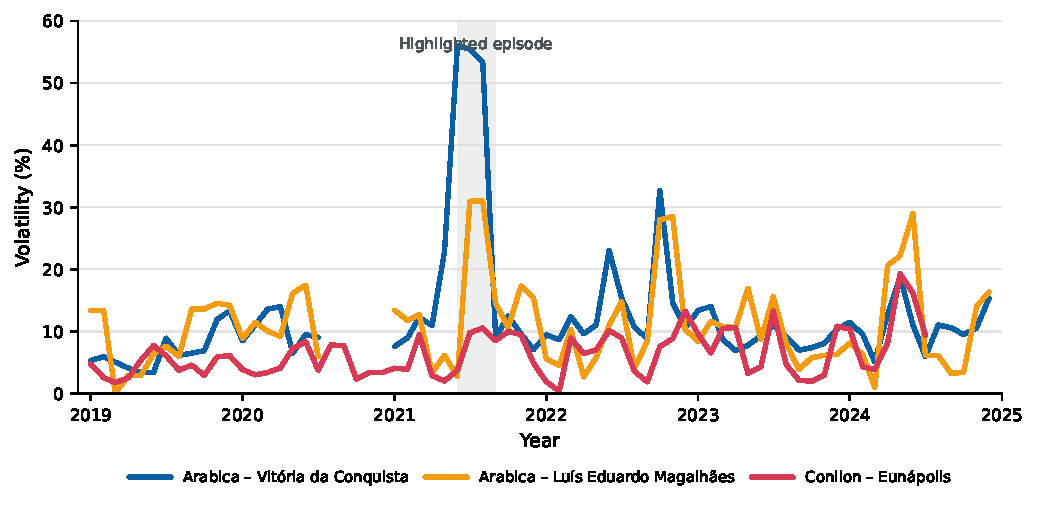
\includegraphics[width=\linewidth]{figs/coffee_bahia_volatility_intro.pdf}
\par\medskip
\noindent\textbf{Figure~\thefigure.} Observed upper-tail volatility of local coffee prices in Bahia, Brazil.
\end{minipage}
\end{center}
\label{fig:intro_volatility}

Diante dessa lacuna, o \textbf{objetivo} deste estudo é avaliar se informações de outras commodities agrícolas e dos mercados financeiros melhoram a previsão fora da amostra da volatilidade futura dos preços locais de café Arábica e Conilon na Bahia, em relação a modelos que utilizam apenas o histórico da própria praça. A análise utiliza três séries locais da SEAGRI-BA, correspondentes ao café Arábica em Vitória da Conquista, ao café Arábica em Luís Eduardo Magalhães e ao café Conilon em Eunápolis. Para atingir esse objetivo, o estudo responde a seis perguntas de pesquisa:

\begin{itemize}
\item[\textbf{RQ1.}] Os modelos de machine learning apresentam desempenho superior aos modelos econométricos tradicionais (GARCH e HAR-RV) na previsão da volatilidade local do café?
\item[\textbf{RQ2.}] A inclusão de informações de outras commodities (café internacional, indicador CEPEA, soja, algodão e cacau) melhora a previsão em relação ao histórico próprio?
\item[\textbf{RQ3.}] Variáveis financeiras e macrofinanceiras (câmbio, juros, petróleo, volatilidade financeira e índices acionários) fornecem ganho preditivo adicional?
\item[\textbf{RQ4.}] O desempenho relativo dos modelos e o valor da informação externa diferem entre regimes de baixa, média e alta volatilidade?
\item[\textbf{RQ5.}] Quais variáveis e blocos de informação mais contribuem para as previsões de cada variedade?
\item[\textbf{RQ6.}] Os fatores relevantes são semelhantes entre Arábica e Conilon ou específicos de cada variedade?
\end{itemize}

As perguntas são tratadas como uma avaliação empírica fora da amostra, sem pressupor a direção dos efeitos. Resultados nulos ou negativos são, portanto, informativos para a seleção de modelos e de fontes de informação. RQ1 compara famílias de modelos; RQ2 e RQ3 isolam o valor de cada bloco de informação; RQ4 examina a estabilidade desses resultados; e RQ5 e RQ6 identificam os fatores associados às previsões.

O desenho empírico compara GARCH(1,1) e HAR-RV com Random Forest, XGBoost e LightGBM, estimados sobre quatro conjuntos de informação aninhados. E1 utiliza apenas o histórico próprio, E2 acrescenta variáveis cross-commodity, E3 acrescenta variáveis financeiras e E4 reúne todos os blocos. Essa estrutura separa o efeito do algoritmo do efeito da informação. A avaliação utiliza validação temporal estrita em janela crescente, horizontes de uma, cinco e vinte observações, as perdas QLIKE, MAE e RMSE, testes de Diebold--Mariano com correção de Harvey--Leybourne--Newbold e correção para múltiplas comparações, análise por regimes definidos ex ante e explicabilidade por importâncias nativas e SHAP \citep{Wang2024SystemicRiskML,Diachkov2026FinancialStressML}.

O estudo oferece três contribuições. Primeiro, fornece evidência fora da amostra sobre a previsão da volatilidade de preços locais de café em um mercado emergente, caracterizado por cotações pouco frequentes e longas lacunas, condição pouco explorada pela literatura concentrada em contratos futuros e índices internacionais. Segundo, quantifica o valor incremental de cada bloco de informação por meio de experimentos de ablação controlados, em vez de apenas ordenar algoritmos. Terceiro, mostra que benchmarks econométricos simples permanecem difíceis de superar nesse contexto e que a importância atribuída a variáveis financeiras pelos modelos não se converte em ganho preditivo, um alerta relevante para aplicações de machine learning em finanças agrícolas.

O restante do artigo está organizado da seguinte forma. A Section~\ref{sec:materials_methods} descreve os dados, as medidas de volatilidade, os modelos e o protocolo de validação. A Section~\ref{sec:experiments} apresenta os experimentos e seus resultados, organizados pelas perguntas de pesquisa. A Section~\ref{sec:discussion} discute os resultados à luz da literatura e apresenta as limitações, e a Section~\ref{sec:conclusion} conclui.

\section{Materials and Methods}
\label{sec:materials_methods}

Esta seção descreve um desenho observacional em duas camadas. A primeira organiza as cotações locais, as commodities relacionadas e os indicadores financeiros em um painel temporal. A segunda utiliza blocos aninhados de atributos para produzir previsões fora da amostra da volatilidade futura dos preços locais de café com modelos econométricos e de machine learning. Assim, os resultados são interpretados como evidência de conteúdo informacional incremental e não como uma decomposição causal da volatilidade.

\subsection{Desenho do estudo}
\label{subsec:study_design}

O estudo é quantitativo, longitudinal e baseado em séries temporais de preços observados. O desenho empírico combina uma unidade de previsão local com uma representação relacional dos mercados. A unidade de previsão é uma cotação disponível para uma combinação de variedade e praça, identificada por \(c\) e pela data \(t\). Para cada unidade, são observados o preço local, os retornos passados, as medidas históricas de volatilidade, as variáveis externas disponíveis e a volatilidade futura associada ao horizonte \(h\). Formalmente, o conjunto de observações destinado à série \(c\) é

\begin{equation}
\mathcal{D}_{c}=\left\{\left(t,P_{c,t},\mathbf{x}_{c,t},V_{c,t,h}\right)\;\middle|\;t\in\mathcal{T}_{c},\ h\in\{1,5,20\}\right\}.
\label{eq:data_unit}
\end{equation}

\refstepcounter{figure}
\begin{center}
\begin{minipage}{\textwidth}
\centering
\resizebox{\textwidth}{!}{%
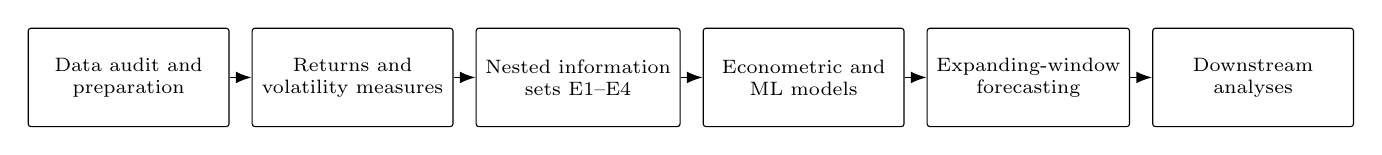
\begin{tikzpicture}[
  stage/.style={draw, rectangle, rounded corners=1pt, minimum width=2.55cm, minimum height=1.25cm, align=center, font=\scriptsize},
  flow/.style={-{Latex[length=2mm]}, line width=0.6pt}
]
\node[stage] (data) {Data audit and\\preparation};
\node[stage, right=0.28cm of data] (temporal) {Returns and\\volatility measures};
\node[stage, right=0.28cm of temporal] (sets) {Nested information\\sets E1--E4};
\node[stage, right=0.28cm of sets] (models) {Econometric and\\ML models};
\node[stage, right=0.28cm of models] (forecast) {Expanding-window\\forecasting};
\node[stage, right=0.28cm of forecast] (downstream) {Downstream\\analyses};
\draw[flow] (data) -- (temporal);
\draw[flow] (temporal) -- (sets);
\draw[flow] (sets) -- (models);
\draw[flow] (models) -- (forecast);
\draw[flow] (forecast) -- (downstream);
\end{tikzpicture}%
}
\noindent\textbf{Figure~\thefigure.} Study workflow: data preparation, volatility measures, nested information sets, model estimation, expanding-window forecasting and downstream analyses.
\end{minipage}
\end{center}
\label{fig:study_design}

O fluxo apresentado na Figure~\ref{fig:study_design} organiza a análise em seis blocos. A preparação dos dados estrutura as observações locais e externas em uma base temporal comum. As medidas de retorno e volatilidade transformam preços em atributos comparáveis entre unidades e definem o alvo de previsão. Os conjuntos de informação aninhados E1--E4 separam o histórico próprio, a informação cross-commodity e a informação financeira. Os modelos econométricos e de machine learning são estimados sobre esses conjuntos, e a previsão em janela crescente produz as estimativas fora da amostra para os horizontes de um, cinco e vinte observações. Por fim, as análises downstream avaliam desempenho preditivo, significância estatística, heterogeneidade entre mercados e regimes e importância das variáveis.

Como as séries locais apresentam dias sem atualização e longos intervalos sem observação, não foi criada uma grade diária artificial. Cada horizonte é contado em observações sucessivas da própria série-alvo. Essa decisão preserva a natureza dos dados e evita transformar períodos sem cotação em retornos sintéticos.

As variáveis dependentes são o café Arábica nas praças de Vitória da Conquista e Luís Eduardo Magalhães e o café Conilon na praça de Eunápolis. Para tornar a comparação internamente consistente, foi selecionado o tipo Rio para as duas séries de Arábica e o tipo 7 para a série de Conilon. Após a limpeza descrita na Seção~\ref{subsec:data_cleaning}, o painel contém 14.126 observações distribuídas entre as três séries.

\begin{table*}[t]
\centering
\caption{Characteristics of the local series used as dependent variables}
\label{tab:target_series}
\scriptsize
\begin{tabular*}{\textwidth}{@{\extracolsep{\fill}}p{3.6cm}lrlrrr@{}}
\hline
Série & Tipo & \(N\) & Período & \(s(r_t)\) & Mediana \(HVol_{5}\) & Mediana \(V_{20}\) \\
\hline
Arábica, Vitória da Conquista & Rio & 4.427 & 2001-12-03 a 2026-01-21 & 3,126 & 2,410 & 6,899 \\
Arábica, Luís Eduardo Magalhães & Rio & 4.195 & 2003-02-05 a 2026-01-21 & 3,066 & 0,000 & 6,899 \\
Conilon, Eunápolis & Tipo 7 & 5.504 & 2001-12-14 a 2026-01-21 & 1,962 & 1,170 & 4,455 \\
\hline
\end{tabular*}
\end{table*}

Os preços são expressos em reais por saca de 60 kg. Os retornos e as medidas \(HVol_{5}\) e \(V_{20}\) estão em pontos percentuais. O horizonte de vinte períodos corresponde às próximas vinte observações disponíveis da série local.

\subsection{Fontes de dados e variáveis observadas}
\label{subsec:data_sources}

Os preços locais foram obtidos da Secretaria da Agricultura, Pecuária, Irrigação, Pesca e Aquicultura da Bahia, identificada como SEAGRI-BA. O preço nacional de referência foi obtido do Centro de Estudos Avançados em Economia Aplicada, com séries de café Arábica e café Robusta. Os contratos futuros internacionais foram obtidos por meio das séries contínuas disponibilizadas pelo Yahoo Finance. Foram utilizados o contrato de café ICE Coffee C \texttt{KC=F}, soja \texttt{ZS=F}, algodão \texttt{CT=F} e cacau \texttt{CC=F}. Essas séries são tratadas como referências de mercado e não como substitutas automáticas de uma série oficial de contratos individuais, pois a convenção de continuidade e de rolagem pertence à fonte de dados.

As variáveis financeiras e macrofinanceiras foram combinadas a partir de fontes públicas. A taxa USD/BRL e a taxa SELIC anualizada para 252 dias foram obtidas do Banco Central do Brasil. O índice de volatilidade VIX, o índice amplo do dólar, a taxa dos títulos do Tesouro dos Estados Unidos com maturidade de dez anos e a taxa efetiva dos Fed Funds foram obtidos do Federal Reserve Economic Data. O preço spot do Brent foi obtido da U.S. Energy Information Administration. Os retornos do S\&P 500 e do Ibovespa foram calculados a partir das séries históricas correspondentes.

\subsubsection{Análise exploratória dos dados}
\label{subsec:eda}

Antes da integração das fontes e da estimação dos modelos, foi realizada uma análise exploratória dos dados em três dimensões. A primeira examinou a cobertura temporal, o número de observações, a mediana dos preços, o desvio-padrão dos retornos e as medidas de volatilidade histórica e futura. Esses resultados são apresentados na Table~\ref{tab:target_series}. O painel final contém 14.126 observações distribuídas entre as três séries locais. As medianas dos preços são 300,00, 310,00 e 247,00 reais por saca de 60 kg para Vitória da Conquista, Luís Eduardo Magalhães e Eunápolis, respectivamente. Os desvios-padrão dos retornos são 3,126, 3,066 e 1,962 pontos percentuais, enquanto as medianas de \(V_{20}\) são 6,899, 6,899 e 4,455 pontos percentuais. A coincidência das medianas de \(V_{20}\) nas duas séries de Arábica decorre da discretização das cotações, que concentra as variações em poucos degraus de preço, e não de séries idênticas. Nas 3.958 datas comuns, os preços das duas praças coincidem em apenas 12,86\% das datas e a correlação entre os retornos é de 0,137, embora os níveis de preço sejam fortemente correlacionados (0,991). Apenas 5,38\% das datas comuns registram variação simultânea de preço nas duas praças.

A segunda dimensão avaliou a frequência efetiva de atualização dos preços. Foram observadas proporções de preços inalterados de 77,48\% em Vitória da Conquista, 87,56\% em Luís Eduardo Magalhães e 84,10\% em Eunápolis. Assim, uma data registrada não representa necessariamente uma nova transação ou uma mudança de preço. Essa baixa frequência de atualização transfere-se para o alvo: no suporte comum de avaliação, a volatilidade futura é exatamente nula em 76,9\% a 88,4\% das origens para \(h=1\), em 36,6\% a 53,0\% para \(h=5\) e em 5,8\% a 10,0\% para \(h=20\), dependendo da série. Essa característica condiciona a avaliação pela QLIKE e é tratada explicitamente nas análises de robustez. A terceira dimensão examinou a evolução da volatilidade ao longo do tempo. A Figure~\ref{fig:intro_volatility} evidencia diferenças entre as praças e destaca o episódio de junho a agosto de 2021, quando o percentil 90 mensal alcançou aproximadamente 56\% em Vitória da Conquista, 31\% em Luís Eduardo Magalhães e 11\% em Eunápolis. O EDA foi utilizado para orientar a definição dos horizontes, a interpretação das lacunas e a escolha de medidas baseadas em observações sucessivas, sem substituir a validação temporal.

\subsubsection{Auditoria dos dados e critérios de retenção}
\label{subsec:data_audit}

A auditoria automatizada foi aplicada a 74 séries candidatas provenientes de SEAGRI-BA, CEPEA, Banco Central do Brasil, Federal Reserve Economic Data, CBOE, U.S. Energy Information Administration e Yahoo Finance. Para cada série foram registrados a fonte, a cobertura temporal, a frequência, o número de observações, a proporção de valores ausentes, as datas duplicadas, a proporção de preços inalterados, o maior intervalo entre observações, a média de observações mensais, a cobertura de dias úteis, alterações de unidade, uma taxa inicial de anomalias e observações sobre a origem dos dados. A triagem genérica classificou 31 séries como inicialmente utilizáveis e 43 como não utilizáveis, principalmente por cobertura insuficiente, lacunas extensas ou inconsistência de unidade.

O indicador de utilização foi tratado como diagnóstico e não como exclusão automática das séries-alvo predefinidas. As três séries locais foram mantidas por sua relevância substantiva para a pergunta de pesquisa, e suas limitações foram incorporadas ao desenho empírico. Os maiores intervalos entre observações foram de 374 dias em Vitória da Conquista, 812 dias em Luís Eduardo Magalhães e 217 dias em Eunápolis. As taxas iniciais de anomalias foram 0,23\%, 0,48\% e 0,25\%, respectivamente. Essas evidências justificaram a não aplicação de interpolação de preços, a contagem dos horizontes em observações sucessivas e a preservação explícita de valores ausentes.

No painel final, a taxa de retorno da série CEPEA apresenta 58,18\% de valores ausentes por iniciar em 2016, enquanto os percentuais de ausência são 0,35\% para o retorno USD/BRL, 2,36\% para o VIX, 1,85\% para o retorno do Brent, 2,79\% para o retorno da soja, 2,96\% para o retorno do algodão e 2,97\% para o retorno do cacau. A informação disponível e o padrão de ausência foram preservados para permitir que a contribuição incremental de cada bloco fosse avaliada sob uma regra comum de amostra e imputação.

\subsection{Limpeza, controle de qualidade e sincronização temporal}
\label{subsec:data_cleaning}

As datas foram convertidas para o formato temporal padrão, os registros foram ordenados e observações duplicadas foram agrupadas por data, mantendo-se a última cotação registrada. Não foi aplicada interpolação linear aos preços. A ausência de uma cotação não foi interpretada como estabilidade de preço e não foi preenchida com uma observação futura.

Foram removidos o dia 1 de janeiro em todos os anos, uma vez que as cotações registradas nessa data eram incompatíveis com um dia regular de negociação, o registro de 31 de agosto de 2023, identificado como uma falha comum do fluxo de dados da SEAGRI-BA, e um ponto isolado de 28 de julho de 2010 na série de Vitória da Conquista, caracterizado por um salto e retorno imediato compatível com erro decimal. Outros retornos absolutos superiores a 40\% foram mantidos e marcados pela variável indicadora \texttt{is\_extreme\_return}. A preservação evita eliminar movimentos potencialmente informativos em um estudo cujo objeto é precisamente a variação extrema.

Cada série exógena foi transformada em seu próprio calendário antes da integração. Para uma data \(t\) da série-alvo, a observação exógena utilizada é

\begin{equation}
x_{j,t}^{*}=x_{j,\tau_j(t)},
\qquad
\tau_j(t)=\max\left\{s\leq t\;|\;t-s\leq 7\text{ dias}\right\}.
\label{eq:asof}
\end{equation}

Quando não existe uma observação \(s\) que satisfaça a condição da Equação~\ref{eq:asof}, o valor permanece ausente. A integração foi realizada por uma junção temporal para trás com tolerância de sete dias. O procedimento utiliza somente a informação disponível até a data de previsão e evita o preenchimento silencioso através de lacunas prolongadas.

\subsection{Retornos e medidas de volatilidade}
\label{subsec:returns_volatility}

Os retornos logarítmicos definem a unidade estatística utilizada para representar a dinâmica dos preços e a variável-alvo da previsão. Eles reduzem o efeito da escala nominal e permitem comparar as praças locais com as commodities e os mercados financeiros. A partir desses retornos, as medidas históricas resumem a intensidade recente das variações e alimentam os modelos com informação disponível na origem \(t\), enquanto a soma de retornos futuros constrói o alvo para cada horizonte. Essa separação entre informação passada e variação futura é fundamental para evitar vazamento temporal e interpretar os ganhos dos blocos adicionais de informação.

Para cada série \(c\), seja \(P_{c,t}>0\) o preço observado na \(t\)-ésima cotação. O retorno logarítmico, expresso em pontos percentuais, é

\begin{equation}
r_{c,t}=100\ln\left(\frac{P_{c,t}}{P_{c,t-1}}\right).
\label{eq:log_return}
\end{equation}

O retorno na primeira observação de cada série é ausente. Para as séries exógenas de preços, a mesma transformação foi aplicada em seus calendários nativos antes da junção temporal.

As medidas históricas de variação utilizadas como atributos foram calculadas exclusivamente com retornos disponíveis até \(t\). Para uma janela \(k\), define-se

\begin{equation}
HVar_{c,t,k}=\sum_{j=0}^{k-1}r_{c,t-j}^{2}
\label{eq:hist_var}
\end{equation}

e

\begin{equation}
HVol_{c,t,k}=\sqrt{HVar_{c,t,k}}.
\label{eq:hist_vol}
\end{equation}

Foram utilizadas as janelas \(k\in\{5,10,20\}\). Essas medidas não são calculadas com retornos futuros e, portanto, podem ser utilizadas como informação disponível no instante \(t\).

A variável dependente representa a intensidade acumulada das variações futuras. Para cada horizonte \(h\in\{1,5,20\}\), define-se a variação quadrática futura

\begin{equation}
Q_{c,t,h}=\sum_{i=1}^{h}r_{c,t+i}^{2}
\label{eq:forward_variance}
\end{equation}

e a volatilidade futura agregada

\begin{equation}
V_{c,t,h}=\sqrt{Q_{c,t,h}}.
\label{eq:forward_vol}
\end{equation}

O índice \(t+i\) representa a próxima observação disponível da série-alvo, e não necessariamente o próximo dia do calendário. Os modelos supervisionados são ajustados diretamente para \(V_{c,t,h}\). A quantidade \(Q_{c,t,h}=V_{c,t,h}^{2}\) é utilizada na avaliação de perdas específicas para variância, especialmente QLIKE. Como as bases utilizadas são predominantemente diárias e não contêm retornos intradiários, o termo volatilidade futura agregada é preferido à interpretação de uma medida clássica de \textit{realized volatility} intradiária.

Em conjunto, essas definições produzem a referência univariada do estudo. O conjunto de variáveis de histórico próprio \(E1\) utiliza os retornos disponíveis, suas defasagens e \(HVol_{c,t,5}\), \(HVol_{c,t,10}\) e \(HVol_{c,t,20}\). Essa especificação constitui o baseline de informação local para medir o ganho incremental de variáveis cross-commodity e financeiras. Em paralelo, GARCH(1,1) e HAR-RV adaptado funcionam como baselines econométricos, pois modelam a volatilidade exclusivamente a partir do histórico local sob hipóteses distintas sobre persistência e agregação temporal. Assim, esta subseção estabelece os preditores históricos, define o alvo futuro e garante a comparabilidade entre horizontes, enquanto as subseções seguintes avaliam se algoritmos e fontes de informação adicionais melhoram essa referência.

\subsection{Construção dos atributos e conjuntos de informação}
\label{subsec:features}

Os atributos da própria série incluem \(r_{c,t}\), cinco defasagens do retorno e as três medidas históricas \(HVol_{c,t,5}\), \(HVol_{c,t,10}\) e \(HVol_{c,t,20}\). Assim, o bloco de histórico próprio contém nove variáveis

\begin{equation}
\mathcal{I}^{L}_{c,t}
=
\left\{
r_{c,t},r_{c,t-1},\ldots,r_{c,t-5},
HVol_{c,t,5},HVol_{c,t,10},HVol_{c,t,20}
\right\}.
\label{eq:local_info}
\end{equation}

O bloco cross-commodity contém o retorno e a volatilidade de cinco períodos da outra variedade local, os retornos e as volatilidades de cinco períodos de soja, algodão e cacau, além dos retornos do contrato internacional de café e do indicador nacional CEPEA

\begin{equation}
\mathcal{I}^{C}_{t}
=
\left\{
r^{other}_{t},HVol^{other}_{t,5},
r^{soy}_{t},HVol^{soy}_{t,5},
r^{cotton}_{t},HVol^{cotton}_{t,5},
r^{cocoa}_{t},HVol^{cocoa}_{t,5},
r^{ICEcoffee}_{t},r^{CEPEA}_{t}
\right\}.
\label{eq:cross_info}
\end{equation}

Para a variável de outra variedade, o retorno do Conilon corresponde à série de Eunápolis e o retorno de Arábica corresponde à média disponível das duas praças de Arábica. A média é calculada no calendário observado antes da junção com a série-alvo.

O bloco financeiro e macrofinanceiro é

\begin{equation}
\begin{aligned}
\mathcal{I}^{F}_{t}
={}&\left\{
r^{USD/BRL}_{t},HVol^{USD/BRL}_{t,5},
SELIC_{t},VIX_{t},\Delta VIX_{t},
r^{Brent}_{t},r^{Dollar}_{t}, \right.\\
&\left. r^{S\&P500}_{t},r^{Ibovespa}_{t},
Treasury10Y_{t},FedFunds_{t}
\right\}.
\end{aligned}
\label{eq:financial_info}
\end{equation}

As quatro especificações de informação são

\begin{equation}
\mathcal{X}^{E1}_{t}=\mathcal{I}^{L}_{c,t}
\label{eq:e1}
\end{equation}

\begin{equation}
\mathcal{X}^{E2}_{t}=\mathcal{I}^{L}_{c,t}\cup\mathcal{I}^{C}_{t}
\label{eq:e2}
\end{equation}

\begin{equation}
\mathcal{X}^{E3}_{t}=\mathcal{I}^{L}_{c,t}\cup\mathcal{I}^{F}_{t}
\label{eq:e3}
\end{equation}

\begin{equation}
\mathcal{X}^{E4}_{t}=\mathcal{I}^{L}_{c,t}\cup\mathcal{I}^{C}_{t}\cup\mathcal{I}^{F}_{t}.
\label{eq:e4}
\end{equation}

E1 representa o histórico próprio. E2 acrescenta informação cross-commodity. E3 acrescenta informação financeira. E4 contém todos os blocos. Essa estrutura permite estimar o ganho marginal de cada fonte sem confundir a comparação entre algoritmos com a comparação entre conjuntos de informação.

\subsection{Modelos econométricos de referência}
\label{subsec:econometric_models}

Os modelos econométricos fornecem as referências para avaliar o desempenho dos modelos de machine learning. Eles oferecem uma representação controlada da previsibilidade da volatilidade baseada exclusivamente no histórico local, sem utilizar variáveis cross-commodity ou indicadores financeiros. O GARCH(1,1) representa a persistência da variância condicional, o EGARCH é utilizado como análise de robustez para permitir respostas assimétricas a choques positivos e negativos, e o HAR-RV adaptado representa a agregação da variação em escalas diária, semanal e mensal. Todos são estimados com a mesma definição de alvo e sob o mesmo protocolo de validação temporal aplicado aos demais modelos. Essa organização permite distinguir o ganho associado à informação adicional do ganho associado à flexibilidade algorítmica. GARCH(1,1) e HAR-RV constituem as referências principais, enquanto o EGARCH amplia a análise para a assimetria da volatilidade.

\subsubsection{GARCH}

O modelo GARCH(1,1) foi estimado sobre o retorno local com média condicional zero e inovações normais \citep{Bollerslev1986GARCH}

\begin{equation}
r_{c,t}=\sigma_{c,t}z_{c,t},
\qquad
z_{c,t}\sim\mathcal{N}(0,1).
\label{eq:garch_return}
\end{equation}

A variância condicional é

\begin{equation}
\sigma_{c,t}^{2}
=
\omega
+\alpha r_{c,t-1}^{2}
+\beta\sigma_{c,t-1}^{2}.
\label{eq:garch}
\end{equation}

Os parâmetros são estimados no conjunto de treinamento de cada janela anual. A previsão da variação quadrática futura é obtida pela soma das variâncias condicionais previstas

\begin{equation}
\widehat{Q}^{GARCH}_{c,t,h}
=
\sum_{i=1}^{h}\widehat{\sigma}_{c,t+i\mid t}^{2},
\qquad
\widehat{V}^{GARCH}_{c,t,h}
=
\sqrt{\widehat{Q}^{GARCH}_{c,t,h}}.
\label{eq:garch_forecast}
\end{equation}

\subsubsection{EGARCH}

Para representar possíveis respostas assimétricas a choques positivos e negativos, foi estimado um EGARCH(1,1,1) \citep{Nelson1991EGARCH}

\begin{equation}
\ln\left(\sigma_{c,t}^{2}\right)
=
\omega
+\beta\ln\left(\sigma_{c,t-1}^{2}\right)
+\alpha\left(\lvert z_{c,t-1}\rvert-\mathbb{E}\lvert z_{c,t-1}\rvert\right)
+\gamma z_{c,t-1}.
\label{eq:egarch}
\end{equation}

O parâmetro \(\gamma\) permite que choques com sinais distintos produzam efeitos diferentes sobre a volatilidade. Para \(h>1\), as previsões EGARCH foram obtidas por simulação de Monte Carlo com 1.000 trajetórias e semente 42. O EGARCH foi tratado como análise de robustez econométrica. A comparação primária e os testes de superioridade preditiva utilizam somente previsões com suporte comum e excluem o EGARCH quando sua cobertura não é completa.

\subsubsection{HAR-RV adaptado}

O baseline HAR-RV foi implementado como uma regressão linear da volatilidade futura agregada sobre medidas de variação em escalas diária, semanal e mensal \citep{Corsi2009HAR}

\begin{equation}
V_{c,t,h}
=
\beta_{0,h}
+\beta_{d,h}\lvert r_{c,t}\rvert
+\beta_{w,h}HVol_{c,t,5}
+\beta_{m,h}HVol_{c,t,20}
+\varepsilon_{c,t,h}.
\label{eq:har}
\end{equation}

Os coeficientes foram obtidos por mínimos quadrados ordinários exclusivamente no treinamento de cada janela. A especificação é uma adaptação do princípio HAR para a medida de volatilidade agregada disponível nas séries diárias. Foram exigidas pelo menos 250 observações de treinamento para estimar cada baseline.

\subsection{Modelos de machine learning}
\label{subsec:ml_models}

Os modelos supervisionados estimam a volatilidade futura a partir dos conjuntos de informação \(E1\)--\(E4\). A escolha de métodos baseados em árvores decorre da natureza tabular, heterogênea e potencialmente não linear dos atributos, que combinam retornos, medidas de volatilidade, preços de commodities e indicadores financeiros. Esses modelos também permitem representar interações sem impor uma forma funcional linear e não exigem escalonamento das variáveis, o que reduz transformações desnecessárias em uma base com diferentes unidades e frequências de atualização.

O Random Forest foi incluído como referência de agregação por \textit{bagging}. A média de várias árvores reduz a instabilidade de uma árvore individual e oferece uma referência robusta para relações não lineares e observações extremas. O XGBoost foi escolhido como método de \textit{boosting} gradiente, no qual árvores sucessivas corrigem os erros das anteriores e podem capturar interações mais concentradas entre os preditores. O LightGBM amplia essa comparação com uma implementação de \textit{boosting} baseada em histogramas e crescimento eficiente das árvores. A inclusão dos dois métodos de \textit{boosting} permite verificar se o resultado depende de uma implementação específica ou se permanece consistente entre algoritmos com diferentes mecanismos de construção. Em conjunto, os três modelos oferecem um contraste entre redução de variância, aprendizagem sequencial de resíduos e eficiência computacional \citep{Breiman2001RandomForest,ChenGuestrin2016XGBoost,Ke2017LightGBM}.

Para cada conjunto de informação, horizonte e série-alvo, foi ajustado um modelo independente. Essa organização evita que a distribuição da volatilidade de uma praça seja utilizada para ajustar diretamente outra e permite avaliar se a contribuição dos atributos se mantém nos horizontes de um, cinco e vinte períodos. Os hiperparâmetros foram fixados para controlar a complexidade, preservar a reprodutibilidade e evitar que o número reduzido de observações por série favorecesse árvores excessivamente profundas. No Random Forest, foram utilizados 100 estimadores, profundidade máxima 6 e mínimo de 5 observações por folha. O número de árvores estabiliza a média do ensemble, a profundidade permite interações de ordem moderada e o tamanho mínimo da folha suaviza previsões em regiões com poucas observações.

Nos modelos de \textit{boosting}, foram utilizados 300 estimadores e taxa de aprendizagem 0,05. O número maior de etapas combinado com atualizações pequenas permite construir a previsão gradualmente e reduz a dependência de correções muito agressivas. Para o XGBoost, a profundidade máxima foi 4, enquanto para o LightGBM foi 5. Essa diferença preserva uma complexidade moderada em ambos os casos, considerando suas formas distintas de crescimento. No LightGBM, foi adicionalmente exigido um mínimo de 10 observações por folha, o que reduz a formação de regiões muito específicas. O estado aleatório foi fixado em 42 em todos os modelos. Não foi aplicado escalonamento, pois as decisões das árvores dependem de pontos de corte e não da distância numérica entre as variáveis.

A Figure~\ref{fig:tree_ml_workflow} mostra o fluxo comum dos modelos baseados em árvores. Cada algoritmo recebe os conjuntos de atributos estruturados \(E1\)--\(E4\) e é estimado de forma independente, de modo que as diferenças de desempenho possam ser atribuídas ao algoritmo ou ao bloco de informação.

\refstepcounter{figure}
\begin{center}
\begin{minipage}{\textwidth}
\centering
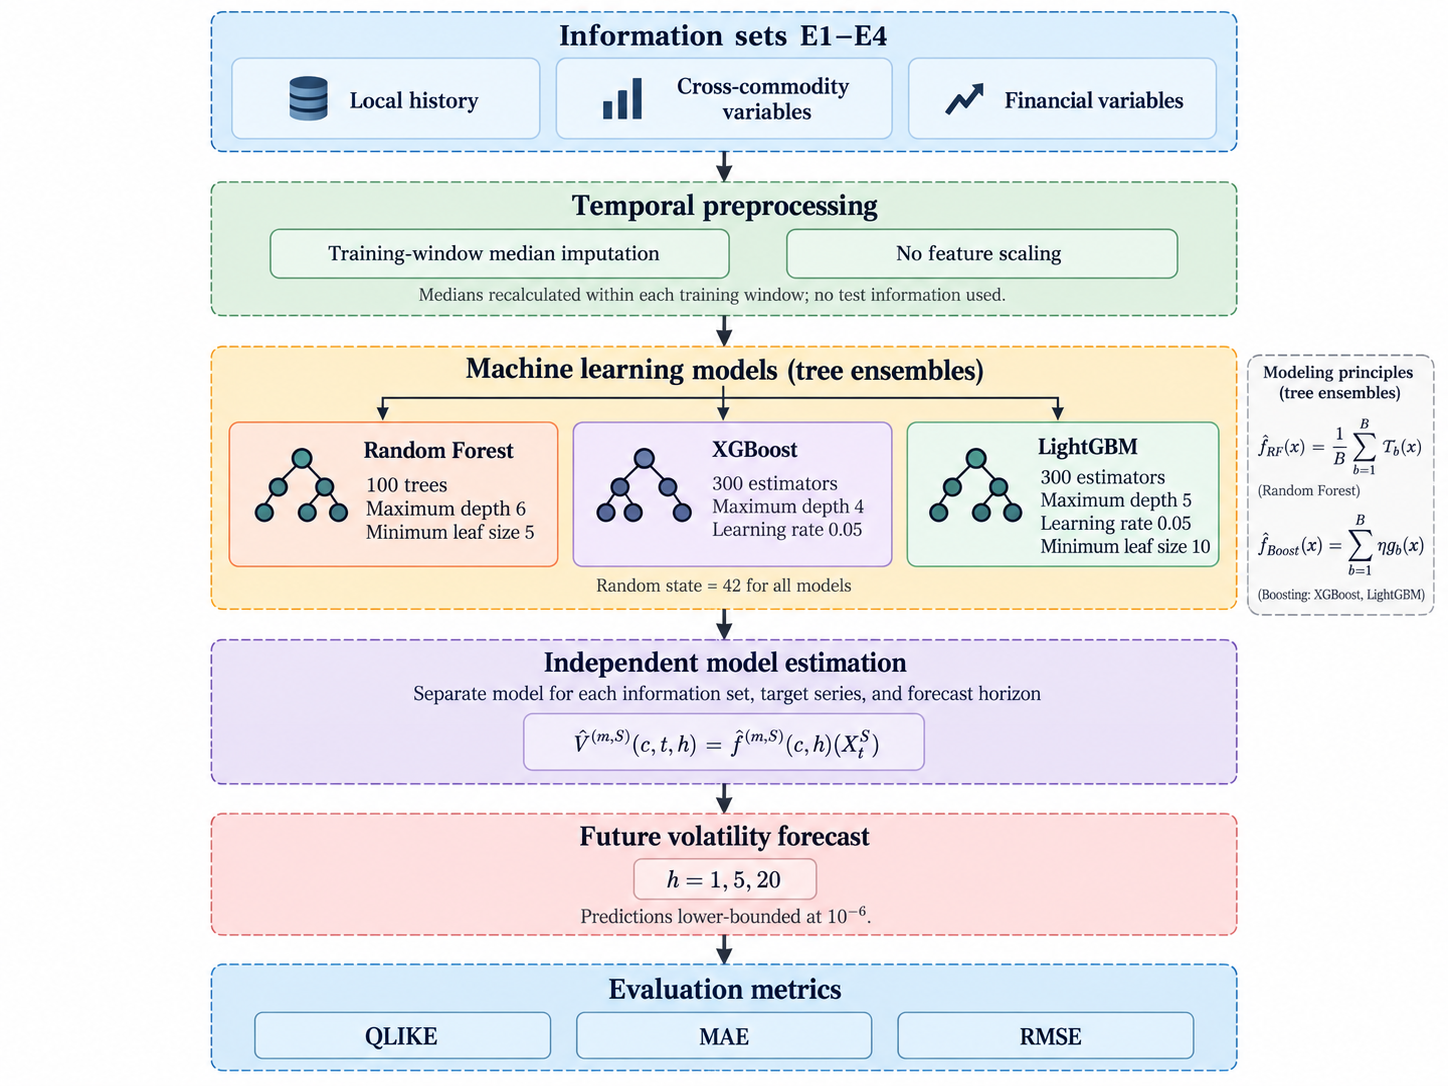
\includegraphics[width=\textwidth]{figs/ml.png}
\par\medskip
\noindent\textbf{Figure~\thefigure.} Workflow of the tree-based machine learning models for local coffee volatility forecasting.
\end{minipage}
\end{center}
\label{fig:tree_ml_workflow}

Para cada conjunto de informação \(S\), horizonte \(h\) e algoritmo \(m\), foi estimada uma função

\begin{equation}
\widehat{V}^{m,S}_{c,t,h}
=
\widehat{f}^{m,S}_{c,h}\left(\mathcal{X}^{S}_{t}\right).
\label{eq:ml_general}
\end{equation}

Foram utilizados três modelos baseados em árvores \citep{Breiman2001RandomForest,ChenGuestrin2016XGBoost,Ke2017LightGBM}. O Random Forest combina \(B\) árvores de regressão

\begin{equation}
\widehat{f}_{RF}(\mathbf{x})
=
\frac{1}{B}\sum_{b=1}^{B}T_b(\mathbf{x}),
\label{eq:rf}
\end{equation}

enquanto os modelos de boosting formam uma função aditiva

\begin{equation}
\widehat{f}_{Boost}(\mathbf{x})
=
\sum_{b=1}^{B}\eta g_b(\mathbf{x}),
\label{eq:boost}
\end{equation}

em que \(g_b\) é uma árvore adicionada sequencialmente e \(\eta\) é a taxa de aprendizagem.

Os valores ausentes dos atributos foram imputados pela mediana do conjunto de treinamento. Para cada variável \(j\), a transformação foi

\begin{equation}
x^{imp}_{j,t}
=
\begin{cases}
x_{j,t}, & \text{se }x_{j,t}\text{ está observado} \\
\operatorname{mediana}\left(x_{j,t}\mid t\in\mathcal{T}_{train}\right), & \text{se }x_{j,t}\text{ está ausente}.
\end{cases}
\label{eq:imputation}
\end{equation}

Os valores de mediana foram recalculados em cada janela e nunca foram estimados com observações do teste. As previsões foram limitadas inferiormente a \(10^{-6}\) para garantir uma quantidade positiva na transformação para variância.

\subsection{Validação temporal e prevenção de data leakage}
\label{subsec:temporal_validation}

As previsões foram avaliadas por validação temporal com janela de treinamento crescente e reestimação anual. Para um ano de teste \(y\), o ponto de corte é

\begin{equation}
C_y=\text{1 de janeiro do ano }y.
\label{eq:cutoff}
\end{equation}

O conjunto de treinamento para o horizonte \(h\) é

\begin{equation}
\mathcal{T}_{y,h}
=
\left\{
t
\;\middle|\;
\text{date}_{c,t}<C_y,\;
\text{date}_{c,t+h}<C_y,\;
V_{c,t,h}\text{ observado}
\right\}.
\label{eq:train_set}
\end{equation}

O conjunto de teste é

\begin{equation}
\mathcal{E}_{y,h}
=
\left\{
t
\;\middle|\;
\text{ano}(\text{date}_{c,t})=y,\;
V_{c,t,h}\text{ observado}
\right\}.
\label{eq:test_set}
\end{equation}

Essa regra elimina do treinamento os rótulos cujo período futuro alcança o ano de teste. A primeira previsão de cada série ocorre depois de pelo menos três anos completos de histórico e cada ajuste exige no mínimo 250 observações válidas. Para o GARCH e o EGARCH, os parâmetros são estimados uma vez por janela anual e mantidos fixos durante o ano de teste. A recursão da variância é atualizada em cada origem com retornos observados até \(t\), sem alterar os parâmetros estimados. Para HAR-RV e para os modelos de machine learning, o ajuste é igualmente realizado somente com as observações do treinamento.

O mesmo princípio temporal foi aplicado à preparação dos dados. A junção temporal, a imputação e o ajuste de cada algoritmo são executados dentro de cada janela. A comparação final utiliza datas comuns a todas as configurações primárias, de modo que uma diferença de desempenho não seja produzida por amostras de teste distintas. A validação comum reúne 12.541 previsões para \(h=1\), 12.529 para \(h=5\) e 12.484 para \(h=20\).

\subsection{Métricas de previsão}
\label{subsec:metrics}

A qualidade das previsões será comparada entre modelos, conjuntos de informação, séries-alvo e horizontes. A escolha de mais de uma medida é necessária porque a volatilidade futura é avaliada em duas escalas relacionadas, mas não equivalentes. A escala da variância é apropriada para verificar a qualidade da previsão do risco quadrático, enquanto a escala da volatilidade preserva a unidade de interpretação dos retornos acumulados. A tabela resume a função de cada métrica e sua relação com as perguntas empíricas do estudo.

\begin{table*}[t]
\centering
\caption{Forecast evaluation metrics and analytical indicators used in the study}
\label{tab:forecast_metrics}
\scriptsize
\setlength{\tabcolsep}{2pt}
\begin{tabular*}{\textwidth}{@{\extracolsep{\fill}}p{1.8cm}p{2.4cm}p{4.7cm}p{6.1cm}@{}}
\hline
Métrica & Escala e direção & O que privilegia & Questão respondida no estudo \\
\hline
QLIKE & Variância \(Q=V^{2}\), menor é melhor & Avalia a previsão da variância por meio do erro relativo entre \(Q\) e \(\widehat{Q}\). É a medida principal para comparar previsões de risco quadrático. & Qual modelo representa melhor a intensidade do risco futuro quando o alvo é tratado como uma medida de variância e qual informação reduz mais essa perda? \\
\hline
MAE & Volatilidade, menor é melhor & Mede o erro absoluto médio na mesma escala de \(V\). Oferece uma interpretação direta do erro típico e é menos sensível a grandes desvios isolados. & Qual modelo produz previsões mais próximas da volatilidade observada em termos médios e quais resultados permanecem interpretáveis na unidade do fenômeno? \\
\hline
RMSE & Volatilidade, menor é melhor & Eleva ao quadrado os erros antes da média e atribui maior peso a falhas grandes. É especialmente informativa para episódios de estresse e subestimações severas. & Qual modelo reduz melhor os erros extremos e mantém desempenho nos períodos de maior risco? \\
\hline
Ganhos incrementais \(G_C\), \(G_F\) e \(G_{CF}\) & Redução relativa da perda, maior é melhor & Compara a perda do baseline com a perda após acrescentar informação cross-commodity, financeira ou combinada. & A informação externa acrescenta previsibilidade além do histórico próprio? \\
\hline
\end{tabular*}
\end{table*}

A literatura de avaliação de volatilidade mostra que não existe uma ordenação universal dos modelos independente da função de perda. Hansen e Lunde demonstram que a classificação pode ser inconsistente quando uma proxy inadequada é usada para representar a variância condicional e recomendam avaliações fora da amostra com medidas de volatilidade mais informativas \citep{HansenLunde2006ConsistentRanking}. Patton mostra que a comparação pode ser distorcida quando a proxy de volatilidade é imperfeita e identifica uma classe de perdas robustas a esse ruído, na qual a QLIKE ocupa posição central \citep{Patton2011VolatilityProxy}. Revisões de previsão de commodities agrícolas também indicam que os resultados dependem do horizonte, da frequência, da especificação do modelo e do protocolo de validação \citep{Guindani2024AgriculturalForecasting}. Esses resultados fundamentam o uso conjunto de QLIKE, MAE e RMSE neste estudo.

Para cada previsão, sejam \(V_{c,t,h}\) a volatilidade observada, \(\widehat{V}_{c,t,h}\) a previsão, \(Q_{c,t,h}=V_{c,t,h}^{2}\) a variância observada e \(\widehat{Q}_{c,t,h}=\widehat{V}_{c,t,h}^{2}\) a variância prevista. A perda QLIKE foi calculada como

\begin{equation}
\operatorname{QLIKE}_{c,t,h}
=
\frac{Q_{c,t,h}}{\widehat{Q}_{c,t,h}}
-\ln\left(\frac{Q_{c,t,h}}{\widehat{Q}_{c,t,h}}\right)-1.
\label{eq:qlike}
\end{equation}

Como existem observações com retorno zero e, consequentemente, \(Q_{c,t,h}=0\), tanto a variância observada quanto a prevista foram limitadas inferiormente por \(\epsilon=10^{-4}\) antes da aplicação da Equação~\ref{eq:qlike}. Como a proporção de alvos nulos é elevada, especialmente em \(h=1\), o piso pode dominar o valor da perda nessas observações. Por isso, a ordenação dos modelos pela QLIKE foi reavaliada em dois exercícios de robustez: (i) variando o piso em \(\epsilon\in\{10^{-4},10^{-2},10^{-1},1\}\) e (ii) restringindo a avaliação às origens com \(Q_{c,t,h}>0\), nas quais o piso não afeta a variância observada. Os ganhos incrementais também foram recalculados sobre as perdas pooled, isto é, pela razão entre as perdas médias agregadas, o que evita que razões extremas de uma única série dominem a média. A métrica QLIKE é a medida principal para avaliar previsões de variância, enquanto MAE e RMSE são calculados na escala de volatilidade

\begin{equation}
\operatorname{MAE}
=
\frac{1}{n}\sum_{t=1}^{n}
\left\lvert V_{c,t,h}-\widehat{V}_{c,t,h}\right\rvert
\label{eq:mae}
\end{equation}

e

\begin{equation}
\operatorname{RMSE}
=
\sqrt{
\frac{1}{n}\sum_{t=1}^{n}
\left(V_{c,t,h}-\widehat{V}_{c,t,h}\right)^{2}
}.
\label{eq:rmse}
\end{equation}

Para medir a previsibilidade incremental, seja \(R_S\) a perda média fora da amostra para o conjunto \(S\). O ganho relativo de adicionar informação cross-commodity, informação financeira e os dois blocos é

\begin{equation}
G_C=\frac{R_{E1}-R_{E2}}{R_{E1}},
\qquad
G_F=\frac{R_{E1}-R_{E3}}{R_{E1}},
\qquad
G_{CF}=\frac{R_{E1}-R_{E4}}{R_{E1}}.
\label{eq:incremental_gain}
\end{equation}

Também são calculados os ganhos condicionais

\begin{equation}
G_{C\mid F}=\frac{R_{E3}-R_{E4}}{R_{E3}},
\qquad
G_{F\mid C}=\frac{R_{E2}-R_{E4}}{R_{E2}}.
\label{eq:conditional_gain}
\end{equation}

Valores positivos indicam redução da perda média e valores negativos indicam piora da previsão após a inclusão do bloco de informação. A interpretação é preditiva e não causal.

As três métricas respondem a dimensões complementares da pergunta de pesquisa. A QLIKE identifica se um modelo estima adequadamente o risco em termos de variância, a MAE mostra a proximidade média na escala de volatilidade e a RMSE revela se o modelo falha principalmente em episódios de grande amplitude. A comparação entre E1 e E2, E3 e E4 verifica se os blocos cross-commodity e financeiro aumentam a previsibilidade além do histórico local. As diferenças entre modelos, horizontes e séries mostram se esses ganhos são estáveis ou dependem da praça e do período analisado. Nenhuma dessas medidas identifica causalidade, pois todas avaliam capacidade preditiva fora da amostra.

\subsection{Testes de comparação preditiva}
\label{subsec:dm_test}

A comparação preditiva verifica se as diferenças observadas nas métricas de previsão são suficientemente grandes para serem distinguidas da variação amostral. A comparação de duas perdas médias pode sugerir que uma configuração é melhor, mas essa diferença pode não se repetir em outras amostras de teste. O teste de Diebold--Mariano avalia a hipótese de igualdade de acurácia preditiva média entre duas configurações, enquanto a correção de Harvey--Leybourne--Newbold ajusta a inferência em amostras finitas e em situações nas quais os erros de previsão apresentam dependência serial \citep{DieboldMariano1995,HarveyLeybourneNewbold1997}.

Essa correção é particularmente importante neste estudo porque os alvos de cinco e vinte períodos são construídos com retornos futuros sobrepostos. Previsões iniciadas em datas próximas podem compartilhar parte do mesmo intervalo futuro e, por isso, seus diferenciais de perda não são independentes. A estimação da variância com autocovariâncias até \(h-1\) e pesos de Bartlett reduz o risco de declarar superioridade estatística com base em erros-padrão subestimados. Os testes são aplicados separadamente para cada série, horizonte, par de configurações e função de perda, sempre nas datas comuns às previsões comparadas.

Para comparar duas configurações \(A\) e \(B\), definem-se os erros de volatilidade

\begin{equation}
e^{A}_{t}=V_{c,t,h}-\widehat{V}^{A}_{c,t,h},
\qquad
e^{B}_{t}=V_{c,t,h}-\widehat{V}^{B}_{c,t,h}.
\label{eq:forecast_errors}
\end{equation}

Para as perdas de erro quadrático, erro absoluto e QLIKE, a diferença de perdas é, respectivamente,

\begin{equation}
d_t^{SE}=(e^{A}_{t})^{2}-(e^{B}_{t})^{2},
\label{eq:dm_se}
\end{equation}

\begin{equation}
d_t^{AE}=\lvert e^{A}_{t}\rvert-\lvert e^{B}_{t}\rvert
\label{eq:dm_ae}
\end{equation}

e

\begin{equation}
d_t^{QLIKE}
=
\ell^{QLIKE}_{A,t}-\ell^{QLIKE}_{B,t}.
\label{eq:dm_qlike}
\end{equation}

A hipótese nula estabelece igualdade de acurácia preditiva média \citep{DieboldMariano1995,HarveyLeybourneNewbold1997}. Para acomodar a dependência serial associada a horizontes sobrepostos, a variância da média de \(d_t\) foi estimada com autocovariâncias até \(h-1\) e pesos de Bartlett

\begin{equation}
\widehat{\operatorname{Var}}(\bar d)
=
\frac{1}{n}
\left[
\widehat{\gamma}_{0}
+2\sum_{k=1}^{h-1}
\left(1-\frac{k}{h}\right)\widehat{\gamma}_{k}
\right],
\label{eq:dm_variance}
\end{equation}

em que

\begin{equation}
\widehat{\gamma}_{k}
=
\frac{1}{n}
\sum_{t=k+1}^{n}
(d_t-\bar d)(d_{t-k}-\bar d).
\label{eq:dm_covariance}
\end{equation}

O estatístico de Diebold--Mariano corrigido por Harvey--Leybourne--Newbold é

\begin{equation}
DM_{HLN}
=
\frac{\bar d}{\sqrt{\widehat{\operatorname{Var}}(\bar d)}}
\sqrt{
\frac{n+1-2h+h(h-1)/n}{n}
}.
\label{eq:dm_hln}
\end{equation}

Os valores de probabilidade são bicaudais e calculados com distribuição t de Student com \(n-1\) graus de liberdade. Os testes são feitos nas datas comuns entre as duas configurações comparadas, para cada série, horizonte, modelo e função de perda.

Como o desenho produz 891 comparações, a significância individual a 5\% superestima o número de diferenças genuínas. Por isso, os valores de probabilidade foram também ajustados pelo procedimento de Holm, que controla a taxa de erro familiar, e pelo procedimento de Benjamini--Hochberg, que controla a taxa de falsas descobertas, ambos aplicados ao conjunto completo das 891 comparações \citep{Holm1979,BenjaminiHochberg1995}. Os testes de QLIKE foram repetidos nas origens com \(Q_{c,t,h}>0\).

Os testes impactam diretamente o objetivo de identificar conteúdo informacional incremental e não apenas diferenças numéricas de desempenho. A comparação entre E1 e E2, E3 e E4 verifica se a inclusão de variáveis cross-commodity, financeiras ou dos dois blocos produz uma redução de perda estatisticamente defensável. As comparações entre GARCH, HAR-RV e os modelos de árvores mostram se uma configuração possui vantagem consistente para uma métrica e um horizonte específicos. A rejeição da hipótese nula indica diferença de acurácia preditiva média, mas não estabelece causalidade nem garante superioridade em períodos ou mercados fora da amostra analisada. Por isso, os valores de probabilidade são interpretados conjuntamente com a magnitude dos ganhos, a função de perda, o horizonte e a heterogeneidade entre as praças.

\subsection{Heterogeneidade, explicabilidade e reprodutibilidade}
\label{subsec:additional_analyses}

A análise empírica não se limita à comparação da perda média entre modelos. O desempenho pode variar entre períodos de baixa e alta volatilidade, os atributos que sustentam uma previsão precisam ser identificados e todo o procedimento deve permanecer auditável. Por isso, esta seção reúne três análises complementares. A primeira verifica a heterogeneidade do desempenho entre regimes e períodos de estresse. A segunda examina a contribuição relativa das variáveis e dos blocos de informação. A terceira documenta o ambiente computacional e as regras de execução necessárias para reproduzir os resultados. Em conjunto, essas análises conectam a acurácia preditiva à estabilidade, à interpretação econômica e à confiabilidade do pipeline.

\subsubsection{Regimes de volatilidade e períodos de estresse}
\label{subsec:regimes}

A heterogeneidade do desempenho foi examinada em três regimes de volatilidade. A classificação principal é definida \textit{ex ante}, com base na volatilidade histórica disponível na origem da previsão. Para cada série \(c\) e ano de teste \(y\), sejam \(\tilde q_{33,c,y}\) e \(\tilde q_{66,c,y}\) os percentis 33,33 e 66,67 de \(HVol_{c,s,20}\) calculados somente com as datas \(s<C_y\). O regime da origem \(t\) é

\begin{equation}
Z_{c,t}
=
\begin{cases}
\mathrm{Low}, & HVol_{c,t,20}\leq \tilde q_{33,c,y} \\
\mathrm{Medium}, & \tilde q_{33,c,y}<HVol_{c,t,20}\leq \tilde q_{66,c,y} \\
\mathrm{High}, & HVol_{c,t,20}>\tilde q_{66,c,y}.
\end{cases}
\label{eq:regimes}
\end{equation}

Essa definição utiliza apenas informação disponível na origem e corresponde ao que um usuário poderia observar ao emitir a previsão. Uma classificação baseada na volatilidade futura observada, isto é, nos tercis de \(V_{c,t,h}\), seria condicionada ao próprio desfecho e favoreceria mecanicamente, no tercil alto, os modelos que preveem variâncias elevadas. Essa classificação \textit{ex post} é mantida apenas como decomposição descritiva. Os regimes não são utilizados como atributos e não participam do treinamento.

Para verificar formalmente se o valor da informação externa depende do regime, o diferencial de perdas \(d_t=\ell_{E1,t}-\ell_{Ek,t}\), positivo quando o bloco \(Ek\) melhora a previsão, foi regredido sobre indicadores dos regimes médio e alto, tendo o regime baixo como referência. O coeficiente do regime alto mede a diferença entre o ganho no regime alto e no regime baixo. Os erros-padrão foram estimados pelo método de Newey--West com \(\max(5,h)\) defasagens, para acomodar a dependência serial induzida pela sobreposição dos horizontes e pela baixa frequência de atualização dos preços \citep{NeweyWest1987}. Também foram analisados quatro intervalos históricos, pré-2020, o choque da COVID-19 em 2020, a crise de geada e oferta entre 2021 e 2022 e a normalização posterior a 2023.

\subsubsection{Importância das variáveis e explicabilidade}
\label{subsec:explainability}

A análise de explicabilidade foi aplicada aos experimentos E2 e E4 para os três modelos de árvores e para os horizontes \(h\in\{1,5,20\}\). As importâncias nativas dos modelos de árvores foram registradas para cada atributo e normalizadas dentro de cada ajuste. Para o LightGBM, foi utilizado o explicador baseado em árvores do SHAP \citep{LundbergLee2017SHAP}. Para uma observação \(\mathbf{x}\), a decomposição é

\begin{equation}
f(\mathbf{x})
=
\phi_{0}
+\sum_{j=1}^{p}\phi_{j}(\mathbf{x}),
\label{eq:shap_decomposition}
\end{equation}

em que \(\phi_j(\mathbf{x})\) representa a contribuição do atributo \(j\) para a previsão da observação. A importância global do atributo foi calculada pela média do valor absoluto

\begin{equation}
S_j
=
\frac{1}{n}\sum_{i=1}^{n}
\left\lvert\phi_j(\mathbf{x}_i)\right\rvert
\label{eq:shap_global}
\end{equation}

e normalizada por

\begin{equation}
\widetilde{S}_j
=
\frac{S_j}{\sum_{\ell=1}^{p}S_{\ell}}.
\label{eq:shap_normalized}
\end{equation}

Os modelos de explicabilidade são ajustados sobre as observações válidas disponíveis para cada série e horizonte, com imputação pela mediana da própria amostra descritiva. Essa análise não substitui a avaliação fora da amostra. Ela tem a finalidade de identificar quais variáveis sustentam a previsão e como a importância se distribui entre histórico próprio, informação cross-commodity e variáveis financeiras.

\subsubsection{Implementação e reprodutibilidade}
\label{subsec:reproducibility}

O dataset mestre foi construído em Python 3.12.10. O pipeline utilizou pandas 3.0.5, NumPy 2.5.2, arch 8.0.0, scikit-learn 1.9.0, LightGBM 4.7.0, XGBoost 3.4.1 e shap 0.52.0. A construção do painel, os baselines, os experimentos de machine learning, a validação temporal, os testes estatísticos, a análise de regimes e a explicabilidade foram executados em scripts separados e os resultados foram salvos em arquivos CSV para auditoria. As previsões individuais contêm a data de origem, a data final do horizonte, a última data de treinamento, o ponto de corte e a validade da previsão.

A leitura conjunta dessas três análises responde perguntas que não podem ser resolvidas por uma métrica agregada. A decomposição por regimes verifica se os ganhos de informação e de algoritmo permanecem durante condições calmas, intermediárias e turbulentas, além de permitir a comparação com períodos históricos de choque. A explicabilidade identifica quais variáveis e blocos sustentam as previsões e ajuda a distinguir um ganho associado ao histórico local de um ganho associado às commodities ou às finanças. A documentação computacional assegura que as escolhas de dados, treinamento, validação e avaliação possam ser auditadas e reproduzidas. Assim, o conjunto complementa a pergunta central sobre previsibilidade incremental com evidências sobre estabilidade, mecanismo informacional e confiabilidade dos resultados. Essas análises permanecem preditivas e não devem ser interpretadas como prova de causalidade.

\subsection{Justificativa das escolhas metodológicas}
\label{subsec:methodological_rationale}

A escolha das séries locais decorre da auditoria de cobertura, densidade e consistência. As demais séries locais de soja, algodão e cacau apresentaram lacunas, unidades variáveis ou baixa frequência incompatíveis com seu uso como variável dependente. Por isso, Arábica e Conilon foram mantidos como alvos e soja, algodão e cacau foram utilizados como sinais cross-commodity. A escolha de uma variedade e um tipo por praça reduz a heterogeneidade causada por diferenças de classificação e unidade dentro da mesma localidade.

O uso de retornos logarítmicos reduz a influência da escala nominal dos preços e produz uma medida comparável entre mercados. A construção de \(V_{c,t,h}\) a partir dos próximos retornos observados é adequada às bases disponíveis, pois não atribui granularidade intradiária a uma base predominantemente diária. A utilização de \(h=1\), \(h=5\) e \(h=20\) permite distinguir previsões de curto prazo, aproximadamente semanais e aproximadamente mensais em dias de observação.

GARCH, EGARCH e HAR-RV formam referências econométricas com diferentes hipóteses sobre persistência, assimetria e agregação temporal. Random Forest, LightGBM e XGBoost ampliam a comparação para relações não lineares e interações entre variáveis sem impor uma forma funcional paramétrica. A comparação E1--E4 foi escolhida para separar o efeito do algoritmo do valor informacional dos blocos de dados.

A validação temporal crescente e a purga dos rótulos que alcançam o ano de teste são necessárias porque a previsão de volatilidade usa observações futuras na construção do alvo. A imputação por janela evita que a disponibilidade posterior de uma variável altere artificialmente o treinamento histórico. QLIKE é mantida como métrica central por avaliar previsões na escala de variância, enquanto MAE e RMSE preservam uma leitura direta do erro na escala de volatilidade.

A classificação \textit{ex ante} por tercis da volatilidade histórica e a análise de períodos históricos mostram se o desempenho muda entre condições calmas e turbulentas usando apenas informação disponível na origem, o que evita o viés de condicionar a avaliação ao próprio desfecho. Por fim, SHAP e as importâncias dos modelos são utilizadas porque um ganho preditivo sem indicação das variáveis responsáveis teria interpretação econômica limitada. Em conjunto, essas escolhas mantêm a análise alinhada ao objetivo de medir previsibilidade incremental em mercados locais integrados a mercados agrícolas e financeiros mais amplos.

\section{Experiments and Results}
\label{sec:experiments}

Esta seção descreve a execução empírica do pipeline e apresenta, imediatamente após cada elemento do desenho, os resultados e a discussão correspondentes. O desenho foi organizado para separar três fontes de diferença preditiva. A primeira corresponde à flexibilidade do algoritmo, comparando referências econométricas e modelos de machine learning. A segunda corresponde ao conteúdo informacional, comparando o histórico da própria série com blocos cross-commodity e financeiros. A terceira corresponde à estabilidade da previsão, examinada por horizonte, praça, regime de volatilidade e período de estresse. A unidade experimental é a combinação entre série-alvo, horizonte, data de origem, conjunto de informação e modelo.

A comparação E1--E4 mede se fontes externas acrescentam informação ao histórico local. A comparação entre os algoritmos verifica se relações não lineares produzem vantagem consistente sobre as referências econométricas. Os horizontes, praças e regimes mostram onde essa vantagem permanece ou desaparece. Os testes estatísticos qualificam a magnitude das diferenças e a explicabilidade identifica os blocos associados às previsões.

\subsection{Escopo experimental e matriz de comparação}
\label{subsec:experimental_scope}

Os experimentos utilizaram o dataset mestre com 14.126 observações de três séries locais. Foram consideradas as séries de café Arábica tipo Rio em Vitória da Conquista e Luís Eduardo Magalhães e de café Conilon tipo 7 em Eunápolis. Para cada série, foram geradas previsões para \(h=1\), \(h=5\) e \(h=20\) observações futuras. Cada previsão foi emitida depois do fechamento observado em \(t\), usando apenas atributos disponíveis até essa origem.

A comparação primária foi formada por GARCH(1,1), HAR-RV, Random Forest, LightGBM e XGBoost. O EGARCH(1,1,1) foi executado como verificação de robustez, mas não foi incluído no suporte comum primário devido a falhas de convergência em parte das janelas. Os modelos de machine learning foram combinados com quatro conjuntos de informação aninhados. E1 contém nove atributos de histórico próprio, E2 contém esses atributos e dez atributos cross-commodity, E3 contém o histórico próprio e onze atributos financeiros e E4 reúne os trinta atributos disponíveis dos três blocos. Essa organização produz doze configurações de machine learning e permite atribuir diferenças de desempenho ao algoritmo ou ao bloco de informação acrescentado. Nas tabelas, o rótulo E0 designa os baselines econométricos GARCH(1,1) e HAR-RV, que utilizam apenas o histórico de retornos da própria série.

\begin{table*}[t]
\centering
\caption{Experimental matrix used in the validated comparison}
\label{tab:experimental_matrix}
\scriptsize
\setlength{\tabcolsep}{2pt}
\begin{tabular*}{\textwidth}{@{\extracolsep{\fill}}p{2.0cm}p{3.5cm}p{5.9cm}p{3.6cm}@{}}
\hline
Bloco & Configurações & Implementação & Finalidade \\ 
\hline
Séries e horizontes & Três séries locais e \(h=1,5,20\) & Unidade temporal definida pela próxima observação disponível da série-alvo & Medir heterogeneidade entre praças e horizontes \\ 
\hline
Baselines & GARCH(1,1) e HAR-RV & Estimação anual com janela expansiva e pelo menos 250 observações de treinamento & Fixar referências econométricas para a previsibilidade local \\ 
\hline
Robustez econométrica & EGARCH(1,1,1) & Simulação com semente 42 e exclusão de previsões não convergentes & Verificar se assimetria altera a comparação sem substituir o suporte primário \\ 
\hline
Machine learning & Random Forest, LightGBM e XGBoost & Hiperparâmetros fixados, imputação pela mediana do treinamento e execução determinística com semente 42 & Avaliar relações não lineares e interações entre atributos \\ 
\hline
Informação & E1, E2, E3 e E4 & Nove, dezenove, vinte e trinta atributos, respectivamente & Quantificar ganhos incrementais do histórico próprio, commodities e finanças \\ 
\hline
Avaliação & QLIKE, MAE e RMSE & Datas comuns entre todas as configurações primárias e perdas calculadas por série e horizonte & Comparar risco quadrático, erro típico e falhas de grande amplitude \\ 
\hline
Diagnóstico & DM-HLN, regimes e importância & Testes em três perdas com correções de Holm e Benjamini--Hochberg, regimes \textit{ex ante} com testes HAC, períodos históricos, importâncias nativas e SHAP & Examinar significância, estabilidade e conteúdo informacional \\
\hline
Robustez & Piso da QLIKE e alvos nulos & \(\epsilon\in\{10^{-4},10^{-2},10^{-1},1\}\), avaliação restrita a \(Q>0\) e ganhos sobre perdas pooled & Verificar se a ordenação depende do tratamento dos alvos nulos \\
\hline
\end{tabular*}
\end{table*}

\subsection{Estimação dos modelos e configuração computacional}
\label{subsec:experiment_implementation}

O GARCH(1,1) foi ajustado aos retornos da série-alvo em cada janela anual e suas previsões foram atualizadas recursivamente com os retornos observados até a origem. O HAR-RV foi estimado por mínimos quadrados usando o retorno absoluto diário e medidas históricas em janelas de cinco e vinte observações. O EGARCH seguiu a mesma separação temporal e utilizou 1.000 simulações nos horizontes superiores a um período. Seus parâmetros permaneceram fixos durante cada ano de teste.

Os modelos tabulares foram ajustados separadamente para cada combinação de série, horizonte, conjunto de informação e janela anual. O Random Forest utilizou 100 árvores, profundidade máxima igual a 6 e mínimo de cinco observações por folha. O LightGBM utilizou 300 árvores, profundidade máxima igual a 5, taxa de aprendizagem de 0,05 e mínimo de dez observações por folha. O XGBoost utilizou 300 árvores, profundidade máxima igual a 4 e taxa de aprendizagem de 0,05. Todos os algoritmos utilizaram \texttt{random\_state=42} e uma única unidade de processamento. Não foi realizada otimização de hiperparâmetros nessa etapa. A fixação dos valores mantém constante a complexidade dos modelos e concentra a comparação no efeito do algoritmo e dos conjuntos de informação.

Antes do ajuste, os atributos ausentes foram imputados pela mediana calculada exclusivamente no conjunto de treinamento. A mesma transformação foi aplicada ao conjunto de teste sem recalcular a mediana. As previsões de volatilidade foram limitadas inferiormente por \(10^{-6}\), enquanto o piso \(\epsilon=10^{-4}\) foi aplicado às variâncias na perda QLIKE. Esses controles evitam previsões negativas e problemas numéricos associados a janelas com retornos iguais a zero.

\subsection{Validação temporal, controle de data leakage e cobertura da avaliação}
\label{subsec:experimental_validation}

O protocolo utilizou uma janela de treinamento crescente e um ciclo de teste anual. A primeira janela foi formada após três anos de observações disponíveis e cada ajuste exigiu pelo menos 250 observações válidas. Em cada ano, todos os atributos, imputações e parâmetros supervisionados foram definidos dentro da janela de treinamento. O conjunto de teste permaneceu separado até a geração da previsão.

Como o alvo de horizonte \(h\) utiliza retornos posteriores à origem, o treinamento foi purgado quando a última observação necessária para construir o rótulo alcançava o ano de teste. A auditoria registrou 186 combinações de série, horizonte e ano de teste e removeu 1.578 rótulos potencialmente sobrepostos ao período de avaliação. As previsões individuais conservaram a origem, o final do horizonte, a última data de treinamento, o ponto de corte e o indicador de validade. Essas informações permitiram verificar que nenhum rótulo supervisionado utilizou observações posteriores ao corte.

Foram tentadas 37.554 previsões para cada configuração, somando as três séries e os três horizontes. As configurações primárias apresentaram 100\% de previsões válidas. O EGARCH apresentou 95,26\% de validade agregada, devido a limitações de convergência, e foi mantido fora da comparação primária por essa razão. Para a comparação principal, foram mantidas somente as datas nas quais todas as configurações primárias possuíam previsão válida. O suporte comum reuniu 12.541 datas para \(h=1\), 12.529 para \(h=5\) e 12.484 para \(h=20\), garantindo que as diferenças de erro não fossem produzidas por amostras distintas.

\subsection{Desempenho pooled: baselines vs.\ machine learning}
\label{subsec:results_coverage}

A avaliação foi realizada na escala de volatilidade e na escala de variância. A QLIKE foi calculada com o piso numérico definido na metodologia e recebeu o papel de medida principal para o risco quadrático. MAE mediu a distância absoluta entre a volatilidade observada e a prevista. RMSE atribuiu peso adicional aos erros de grande amplitude. A agregação pooled atribuiu o mesmo peso a cada previsão individual, sobre as 12.541, 12.529 e 12.484 datas do suporte comum descrito na Section~\ref{subsec:experimental_validation}.

A Table~\ref{tab:pooled_results} resume as configurações vencedoras em cada horizonte e função de perda. O GARCH(1,1) apresentou a menor QLIKE nos três horizontes, com valores de 9,374, 6,362 e 2,606. O HAR-RV apresentou o menor MAE e o menor RMSE em todos os horizontes, com MAE de 1,074, 2,783 e 5,254 e RMSE de 2,442, 4,992 e 8,697. Esse resultado mostra que a ordenação dos modelos depende da escala de avaliação. O GARCH foi favorecido quando a comparação priorizou a variância, enquanto o HAR-RV foi favorecido quando o interesse recaiu sobre a distância entre a volatilidade prevista e a observada.

\begin{table}[t]
\centering
\caption{Pooled winning configurations by horizon and loss}
\label{tab:pooled_results}
\scriptsize
\setlength{\tabcolsep}{2pt}
\begin{tabular}{@{}p{0.65cm}p{1.05cm}p{2.55cm}r@{}}
\hline
\(h\) & Perda & Configuração vencedora & Valor \\
\hline
1 & QLIKE & E0--GARCH(1,1) & 9,374 \\
1 & MAE & E0--HAR-RV & 1,074 \\
1 & RMSE & E0--HAR-RV & 2,442 \\
5 & QLIKE & E0--GARCH(1,1) & 6,362 \\
5 & MAE & E0--HAR-RV & 2,783 \\
5 & RMSE & E0--HAR-RV & 4,992 \\
20 & QLIKE & E0--GARCH(1,1) & 2,606 \\
20 & MAE & E0--HAR-RV & 5,254 \\
20 & RMSE & E0--HAR-RV & 8,697 \\
\hline
\end{tabular}
\end{table}

Entre os modelos de machine learning, o Random Forest apresentou o desempenho agregado mais consistente. Para QLIKE, suas melhores configurações foram E2 em \(h=1\), com 20,437, E2 em \(h=5\), com 7,754, e E1 em \(h=20\), com 3,373. Para MAE, E1 foi a melhor configuração em \(h=1\) e \(h=5\), com 1,109 e 2,934, enquanto E2 foi a melhor em \(h=20\), com 5,440. Para RMSE, E2 foi a melhor configuração em \(h=1\) e \(h=20\), com 2,478 e 9,236, e E1 foi a melhor em \(h=5\), com 5,194. Mesmo quando foi o melhor modelo de machine learning, o Random Forest permaneceu acima do HAR-RV em MAE e RMSE pooled. A diferença diminuiu no horizonte de vinte observações, mas não desapareceu.

Os modelos de boosting apresentaram maior instabilidade sob QLIKE. O LightGBM obteve perdas pooled elevadas nos três horizontes, enquanto o XGBoost alternou ganhos relativos em algumas configurações com perdas elevadas em outras. Essa diferença entre as famílias não deve ser interpretada como superioridade universal do Random Forest, pois os resultados dependem da função de perda e da praça. Ela indica que a flexibilidade não paramétrica, isoladamente, não substitui a necessidade de uma referência econométrica adequada à escala do risco.

A Figure~\ref{fig:pooled_comparison} representa graficamente essa comparação pooled, mostrando QLIKE (em escala logarítmica), MAE e RMSE por horizonte para os dois baselines e a melhor configuração de cada família de machine learning. A figura evidencia visualmente a inversão de ordenação entre QLIKE e as métricas de escala de volatilidade e a maior dispersão de LightGBM e XGBoost sob QLIKE.

\refstepcounter{figure}
\begin{center}
\begin{minipage}{\textwidth}
\centering
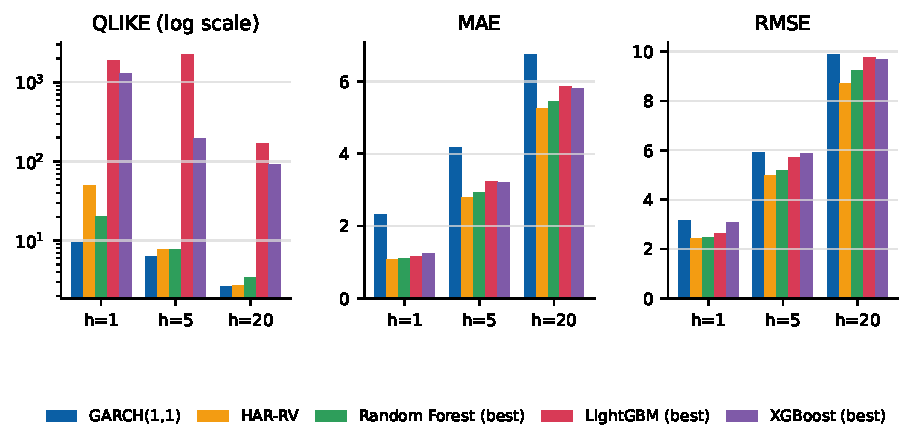
\includegraphics[width=\textwidth]{figs/fig_pooled_comparison.pdf}
\par\medskip
\noindent\textbf{Figure~\thefigure.} Pooled QLIKE, MAE and RMSE by horizon for GARCH(1,1), HAR-RV and the best configuration of each machine-learning family.
\end{minipage}
\end{center}
\label{fig:pooled_comparison}

\subsection{Robustez da QLIKE aos alvos nulos}
\label{subsec:results_qlike_robustness}

Como a volatilidade futura é nula em grande parte das origens, especialmente em \(h=1\), os valores absolutos da QLIKE pooled são elevados e dependem do piso \(\epsilon\). Para verificar se a ordenação dos modelos é um artefato desse piso, a Table~\ref{tab:qlike_robust} reapresenta a QLIKE pooled com \(\epsilon=1\) e restrita às origens com \(Q_{c,t,h}>0\).

\begin{table}[t]
\centering
\caption{QLIKE robustness: pooled QLIKE of GARCH(1,1), HAR-RV and the best machine-learning configuration under alternative variance floors and on non-zero targets}
\label{tab:qlike_robust}
\scriptsize
\setlength{\tabcolsep}{2pt}
\begin{tabular}{@{}p{1.55cm}p{0.4cm}rrrrl@{}}
\hline
Cenário & \(h\) & \(n\) & GARCH & HAR-RV & Melhor ML & Configuração \\
\hline
\(\epsilon=10^{-4}\) & 1 & 12.541 & 9,374 & 49,990 & 20,437 & E2--RF \\
 & 5 & 12.529 & 6,362 & 7,636 & 7,754 & E2--RF \\
 & 20 & 12.484 & 2,606 & 2,688 & 3,373 & E1--RF \\
\hline
\(\epsilon=1\) & 1 & 12.541 & 1,956 & 5,382 & 3,950 & E4--XGB \\
 & 5 & 12.529 & 2,332 & 3,658 & 3,781 & E2--RF \\
 & 20 & 12.484 & 1,888 & 1,970 & 2,656 & E1--RF \\
\hline
\(Q>0\) & 1 & 2.131 & 7,810 & 258,759 & 84,806 & E2--RF \\
 & 5 & 7.033 & 2,518 & 5,629 & 5,846 & E2--RF \\
 & 20 & 11.525 & 1,765 & 1,879 & 2,638 & E1--RF \\
\hline
\end{tabular}
\end{table}

O GARCH(1,1) apresentou a menor QLIKE pooled em todos os cenários e horizontes, inclusive nos valores intermediários \(\epsilon=10^{-2}\) e \(\epsilon=10^{-1}\), não reportados na tabela. A magnitude das perdas diminui à medida que o piso aumenta ou que os alvos nulos são excluídos, mas a ordenação entre GARCH, HAR-RV e o melhor modelo de machine learning permanece inalterada. Nas origens com variação de preço, o GARCH também apresentou o menor MAE e o menor RMSE em \(h=1\), com 2,305 e 5,002, enquanto o HAR-RV manteve as menores perdas de escala de volatilidade em \(h=5\) e \(h=20\). Esse resultado indica que parte da vantagem do HAR-RV em MAE no horizonte curto decorre de previsões baixas nas origens sem variação de preço. Os testes DM-HLN de QLIKE restritos às origens com \(Q_{c,t,h}>0\) confirmam o padrão: nenhuma configuração de machine learning foi significativamente superior ao GARCH ou ao HAR-RV, e 66 das 108 comparações com o GARCH foram significativamente favoráveis ao GARCH. Portanto, a vantagem do GARCH em QLIKE não é um artefato do tratamento dos alvos nulos.

\subsection{Resultados por praça e horizonte}
\label{subsec:results_heterogeneity}

A decomposição por série confirma a heterogeneidade observada no EDA e responde ao objetivo de verificar se a previsibilidade se mantém entre localidades. O GARCH apresentou a menor QLIKE em oito das nove combinações de série e horizonte. A exceção ocorreu em Luís Eduardo Magalhães no horizonte de vinte observações, em que o HAR-RV apresentou QLIKE de 2,488, inferior ao GARCH. O HAR-RV apresentou o menor RMSE nas nove combinações e o menor MAE em oito. A exceção de MAE também ocorreu em Luís Eduardo Magalhães em \(h=20\), quando E2 com Random Forest apresentou MAE de 6,665, contra 6,682 do HAR-RV.

A vantagem das referências econométricas foi mais clara nos horizontes curtos e intermediários para QLIKE. No horizonte longo, a proximidade entre as previsões aumentou em algumas praças e a informação cross-commodity tornou-se competitiva para o Random Forest. Em Luís Eduardo Magalhães, E2 com Random Forest apresentou MAE de 6,665 e RMSE de 9,203 em \(h=20\). Em Vitória da Conquista e Eunápolis, entretanto, o HAR-RV manteve as menores perdas de escala de volatilidade. A diferença entre as praças reforça que a utilidade dos atributos externos não é homogênea e deve ser avaliada por série e horizonte.

\subsection{Valor incremental dos blocos de informação}
\label{subsec:results_incremental}

As comparações incrementais foram calculadas tomando E1 como referência para cada série, horizonte e algoritmo, de modo que o ganho de E2, E3 ou E4 representasse a redução relativa da perda associada ao novo bloco de informação. A comparação E1--E4 foi realizada conforme o desenho experimental e tomou E1 como referência dentro de cada algoritmo, série e horizonte. A informação cross-commodity foi o bloco externo mais consistente para o Random Forest. Como mostra a Table~\ref{tab:rf_incremental}, E2 reduziu a QLIKE do Random Forest em todas as três séries para \(h=1\), em duas séries para \(h=5\) e em apenas uma série para \(h=20\). Na escala de volatilidade, E2 melhorou o MAE em uma série no horizonte curto, em uma no horizonte intermediário e em duas no horizonte longo. O RMSE foi reduzido em duas séries no horizonte curto, em uma no horizonte intermediário e nas três séries no horizonte longo.

\begin{table}[t]
\centering
\caption{Incremental gains from cross-commodity information for Random Forest}
\label{tab:rf_incremental}
\scriptsize
\setlength{\tabcolsep}{2pt}
\begin{tabular}{@{}p{2.15cm}p{0.55cm}rrr@{}}
\hline
Série & \(h\) & QLIKE (\%) & MAE (\%) & RMSE (\%) \\
\hline
Arábica LEM & 1 & 3,94 & -1,02 & -0,20 \\
Arábica LEM & 5 & 8,75 & 3,22 & 2,39 \\
Arábica LEM & 20 & 2,96 & 4,28 & 4,57 \\
Arábica VDC & 1 & 5,57 & 1,70 & 1,08 \\
Arábica VDC & 5 & 1,66 & -2,88 & -4,10 \\
Arábica VDC & 20 & -8,41 & 0,90 & 3,20 \\
Conilon Eunápolis & 1 & 6,40 & -3,34 & 0,18 \\
Conilon Eunápolis & 5 & -1,86 & -2,48 & -1,30 \\
Conilon Eunápolis & 20 & -3,02 & -1,51 & 1,68 \\
\hline
\end{tabular}
\end{table}

Os ganhos médios de E2 para o Random Forest foram de 5,30\% em QLIKE no horizonte curto, 2,85\% no horizonte intermediário e -2,82\% no horizonte longo. Para MAE, os ganhos médios foram -0,89\%, -0,71\% e 1,22\%. Para RMSE, foram 0,35\%, -1,00\% e 3,15\%. Esses valores evidenciam que o acréscimo de commodities relacionadas pode melhorar a previsão em determinados mercados, mas não produz ganho uniforme em todas as métricas.

O bloco financeiro não apresentou uma melhoria sistemática em relação ao histórico próprio. Para o Random Forest, os ganhos médios de E3 foram negativos em QLIKE nos três horizontes e também em MAE e RMSE. O conjunto completo E4 reproduziu esse padrão, com ganhos médios negativos para o Random Forest nas três métricas.

Os resultados de LightGBM e XGBoost mostram que a instabilidade sob QLIKE é mais intensa nos modelos de boosting. A média simples de ganhos relativos por série, utilizada acima para o Random Forest, torna-se pouco informativa para esses modelos, pois uma única série com perda explosiva domina a média. Por isso, a Table~\ref{tab:ml_incremental_pooled} apresenta os ganhos calculados sobre as perdas pooled, isto é, \(1-\bar R_{Ek}/\bar R_{E1}\), em que \(\bar R\) é a perda média agregada das três séries.

\begin{table*}[t]
\centering
\caption{Incremental gains (\%) over E1 computed on pooled losses, by model, information block and horizon (\(\epsilon=10^{-4}\))}
\label{tab:ml_incremental_pooled}
\scriptsize
\setlength{\tabcolsep}{3pt}
\begin{tabular*}{\textwidth}{@{\extracolsep{\fill}}llrrrrrrrrr@{}}
\hline
 & & \multicolumn{3}{c}{QLIKE} & \multicolumn{3}{c}{MAE} & \multicolumn{3}{c}{RMSE} \\
Modelo & Bloco & \(h=1\) & \(h=5\) & \(h=20\) & \(h=1\) & \(h=5\) & \(h=20\) & \(h=1\) & \(h=5\) & \(h=20\) \\
\hline
Random Forest & E2 & 5,59 & 2,42 & -4,20 & -0,63 & -0,59 & 1,43 & 0,47 & -1,33 & 3,29 \\
Random Forest & E3 & -3,42 & -9,77 & -8,20 & -7,46 & -8,78 & -15,08 & -4,04 & -10,04 & -19,66 \\
Random Forest & E4 & 0,01 & -6,60 & -5,64 & -5,78 & -5,32 & -16,73 & -2,51 & -8,28 & -19,50 \\
LightGBM & E2 & -39,13 & 29,01 & -660,67 & -3,01 & -3,16 & 3,50 & -1,74 & -4,43 & 5,37 \\
LightGBM & E3 & -179,37 & -138,98 & 60,30 & -4,77 & -17,54 & -7,16 & -3,33 & -17,82 & -12,28 \\
LightGBM & E4 & -151,52 & -6,77 & -39,47 & -4,68 & -12,12 & -6,01 & -2,70 & -14,24 & -9,82 \\
XGBoost & E2 & 72,21 & 91,53 & -649,28 & 5,76 & 0,65 & 1,40 & 20,43 & 1,84 & 6,24 \\
XGBoost & E3 & 73,16 & 44,42 & -47,13 & -6,18 & -13,14 & -10,84 & 21,73 & -9,36 & -9,75 \\
XGBoost & E4 & 64,21 & 28,61 & -861,13 & -2,66 & -9,07 & -12,40 & 24,20 & -5,63 & -10,71 \\
\hline
\end{tabular*}
\end{table*}

Três padrões emergem. Primeiro, para o Random Forest, o bloco cross-commodity produz ganhos pequenos e de sinal variável, positivos em QLIKE nos horizontes curto e intermediário e em MAE e RMSE no horizonte longo. Segundo, os blocos financeiro e completo pioram o MAE e o RMSE em todos os modelos no horizonte de vinte observações, com perdas entre 6\% e 20\%. Terceiro, os ganhos de QLIKE dos modelos de boosting alternam valores positivos elevados e perdas de várias centenas de por cento. Os ganhos positivos do XGBoost em \(h=1\) e \(h=5\) refletem sobretudo a fragilidade da configuração E1 desse modelo, e não um bom desempenho absoluto, pois nenhuma configuração do XGBoost se aproxima das perdas do GARCH ou do HAR-RV. Restringindo a avaliação às origens com \(Q_{c,t,h}>0\), os padrões se mantêm: o ganho de QLIKE do Random Forest com E2 é de 7,90\%, 5,46\% e -5,86\% nos três horizontes, e os blocos E3 e E4 permanecem negativos em \(h=5\) e \(h=20\). Portanto, apenas o bloco cross-commodity no Random Forest produz ganhos de magnitude estável, ainda que pequenos, e a informação financeira não se traduz em ganho preditivo.

A Figure~\ref{fig:incremental_gains} resume os ganhos do Random Forest por bloco de informação e horizonte, calculados sobre as perdas pooled. O Random Forest é o único modelo cujos ganhos de QLIKE permanecem em uma escala interpretável nos três blocos. O bloco cross-commodity (E2) é o único que preserva ganho médio positivo em QLIKE nos horizontes curto e intermediário, enquanto os blocos financeiro (E3) e completo (E4) produzem perdas médias em praticamente todas as combinações de métrica e horizonte, confirmando que informação adicional não implica necessariamente ganho preditivo.

\refstepcounter{figure}
\begin{center}
\begin{minipage}{\textwidth}
\centering
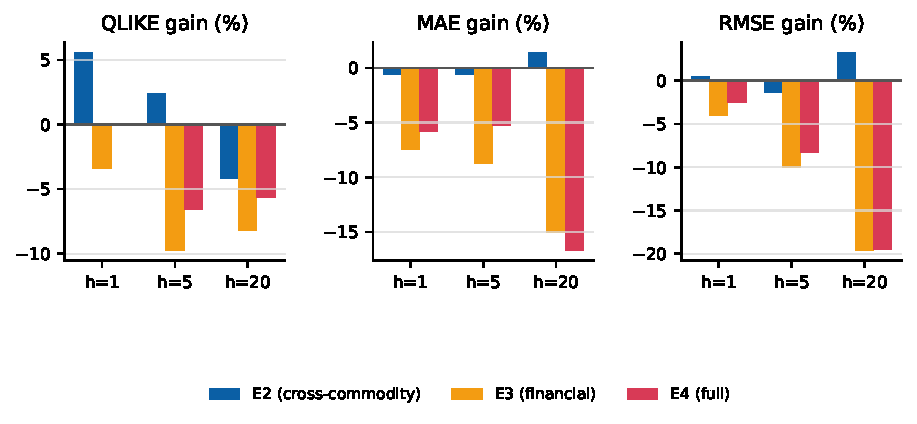
\includegraphics[width=\textwidth]{figs/fig_incremental_gains.pdf}
\par\medskip
\noindent\textbf{Figure~\thefigure.} Incremental gains of Random Forest over the E1 own-history baseline, computed on pooled losses, by information block (E2, E3, E4) and horizon.
\end{minipage}
\end{center}
\label{fig:incremental_gains}

\subsection{Comparações de superioridade preditiva (testes DM-HLN)}
\label{subsec:results_statistical_tests}

As diferenças de desempenho foram submetidas ao teste Diebold-Mariano com a correção de Harvey, Leybourne e Newbold. Foram avaliadas as perdas ao quadrado, as perdas absolutas e a QLIKE. O primeiro conjunto de comparações examinou E1 contra E2, E3 e E4 dentro de cada família de machine learning. O segundo comparou cada configuração de machine learning com HAR-RV e GARCH(1,1). A direção do diferencial foi mantida junto ao valor de probabilidade para distinguir melhoria, empate estatístico e deterioração.

Os testes DM-HLN registrados em \texttt{statistical\_tests\_results.csv} produziram 891 comparações sobre o mesmo suporte temporal utilizado na avaliação, formadas por série, horizonte, par de modelos e função de perda. Dentro das famílias de machine learning, as diferenças entre E1 e os blocos ampliados foram significativas em 54 de 81 comparações de MAE, 53 de 81 comparações de erro quadrático e 10 de 81 comparações de QLIKE. Contudo, somente 13 comparações de MAE e oito de erro quadrático foram significativamente favoráveis ao conjunto ampliado. Nenhuma diferença de QLIKE significativa favoreceu E2, E3 ou E4. Assim, a evidência estatística apoia ganhos incrementais localizados, mas não uma superioridade geral da informação externa.

As comparações com os baselines reforçam a dependência da função de perda. Em QLIKE, nenhuma configuração de machine learning foi significativamente superior ao GARCH ou ao HAR-RV. Em MAE, 88 das 108 comparações entre machine learning e GARCH foram significativamente favoráveis ao modelo de machine learning, enquanto nenhuma comparação com o HAR-RV foi significativamente favorável ao machine learning. Em erro quadrático, 40 comparações foram significativamente favoráveis ao machine learning contra o GARCH e nenhuma contra o HAR-RV. Portanto, os modelos de machine learning conseguem superar o GARCH em parte das comparações na escala de volatilidade, mas não superam o HAR-RV de forma estatisticamente significativa nessa escala.

A Table~\ref{tab:dm_tests} consolida essas 891 comparações DM-HLN em contagens por tipo de comparação e função de perda, com e sem correção para múltiplas comparações.

\begin{table}[t]
\centering
\caption{DM-HLN test outcomes by comparison type and loss function: raw 5\% significance and after Benjamini--Hochberg (BH) and Holm corrections over the 891 tests}
\label{tab:dm_tests}
\scriptsize
\setlength{\tabcolsep}{2pt}
\begin{tabular}{@{}p{2.2cm}p{0.8cm}rrrrrrr@{}}
\hline
 & & & \multicolumn{2}{c}{5\%} & \multicolumn{2}{c}{BH} & \multicolumn{2}{c}{Holm} \\
Comparação & Perda & N & Sig. & Fav. & Sig. & Fav. & Sig. & Fav. \\
\hline
E1 vs.\ E2/E3/E4 & MAE & 81 & 54 & 13 & 49 & 11 & 30 & 2 \\
E1 vs.\ E2/E3/E4 & RMSE & 81 & 53 & 8 & 46 & 6 & 22 & 3 \\
E1 vs.\ E2/E3/E4 & QLIKE & 81 & 10 & 0 & 9 & 0 & 0 & 0 \\
ML vs.\ GARCH(1,1) & MAE & 108 & 94 & 88 & 93 & 87 & 77 & 73 \\
ML vs.\ GARCH(1,1) & RMSE & 108 & 68 & 40 & 60 & 40 & 39 & 32 \\
ML vs.\ GARCH(1,1) & QLIKE & 108 & 65 & 0 & 59 & 0 & 16 & 0 \\
ML vs.\ HAR-RV & MAE & 108 & 94 & 0 & 87 & 0 & 69 & 0 \\
ML vs.\ HAR-RV & RMSE & 108 & 99 & 0 & 96 & 0 & 48 & 0 \\
ML vs.\ HAR-RV & QLIKE & 108 & 43 & 0 & 37 & 0 & 11 & 0 \\
\hline
\end{tabular}
\end{table}

Nas três primeiras linhas, ``Fav.'' conta comparações significativas a favor do conjunto de informação ampliado (E2, E3 ou E4) sobre E1. Nas demais linhas, conta comparações significativas a favor do modelo de machine learning sobre o baseline econométrico correspondente. As diferenças significativas não favoráveis correspondem a deteriorações.

A correção para múltiplas comparações reduz substancialmente a evidência a favor da informação externa. Sob o critério de Holm, que controla a probabilidade de ao menos um falso positivo entre as 891 comparações, restam apenas duas comparações de MAE e três de erro quadrático significativamente favoráveis aos conjuntos ampliados, contra 28 e 19 comparações significativamente desfavoráveis. Sob o critério de Benjamini--Hochberg, menos conservador, restam 11 e 6 comparações favoráveis. Em contraste, a superioridade do HAR-RV sobre os modelos de machine learning e a vantagem do GARCH em QLIKE permanecem após as duas correções. Para o Random Forest com E2, as comparações significativamente favoráveis a 5\% foram 3 de 9 em MAE, 1 de 9 em erro quadrático e nenhuma em QLIKE.

\subsection{Regimes de volatilidade e períodos de estresse}
\label{subsec:results_regimes}

A heterogeneidade foi examinada com regimes definidos \textit{ex ante} pelos tercis da volatilidade histórica \(HVol_{c,t,20}\), com limiares estimados apenas com dados anteriores a cada ano de teste (Equação~\ref{eq:regimes}). O regime baixo concentra 5.730 origens por horizonte, e os regimes médio e alto concentram cerca de 3.500 e 3.300 origens, respectivamente. A assimetria decorre da redução da volatilidade histórica nos anos mais recentes em relação aos limiares estimados com o histórico anterior.

A ordenação entre os modelos permaneceu estável entre os regimes. O GARCH apresentou a menor QLIKE pooled nos três regimes, com 6,336, 5,997 e 5,871 nos regimes baixo, médio e alto, e também nas origens com variação de preço, com 2,426, 2,691 e 2,910. O melhor modelo de machine learning, sempre uma configuração do Random Forest, registrou QLIKE entre 9,799 e 10,722. Em MAE, o HAR-RV foi a melhor referência nos três regimes, com 2,823, 2,908 e 3,535, praticamente empatado com o Random Forest com E2 no regime baixo, com 2,826. Portanto, a vantagem das referências econométricas não depende do regime.

O valor da informação externa, por outro lado, depende fortemente do regime. A Figure~\ref{fig:regime_analysis} apresenta o ganho de MAE de cada bloco sobre E1, calculado sobre as perdas pooled em cada regime. No regime baixo, os blocos financeiro e completo pioram o MAE em 20\% a 27\% em todos os modelos. No regime médio, as perdas diminuem para 2\% a 8\%. No regime alto, os ganhos tornam-se positivos, entre 1,8\% e 7,6\% para E3 e entre 0,7\% e 7,4\% para E4. O bloco cross-commodity, ao contrário, apresenta ganhos pequenos e aproximadamente estáveis entre os regimes, entre -1,7\% e 2,5\%.

\refstepcounter{figure}
\begin{center}
\begin{minipage}{\textwidth}
\centering
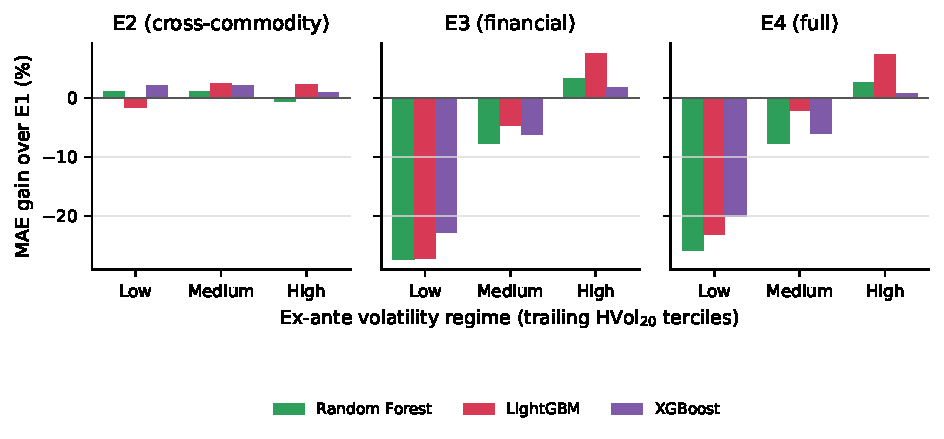
\includegraphics[width=\textwidth]{figs/fig_regime_analysis.pdf}
\par\medskip
\noindent\textbf{Figure~\thefigure.} MAE gain over the E1 own-history baseline by ex-ante volatility regime (terciles of trailing \(HVol_{20}\), thresholds estimated before each test year), by information block and model. Gains are computed on pooled losses.
\end{minipage}
\end{center}
\label{fig:regime_analysis}

Os testes HAC confirmam esse padrão. Para os blocos financeiro e completo, a diferença entre o ganho no regime alto e no regime baixo foi positiva e significativa a 5\% em 6 a 7 das 9 combinações de série e horizonte em MAE para cada modelo, e em 3 a 5 das 9 em erro quadrático, com no máximo uma diferença significativa em sentido contrário. Para o bloco cross-commodity, as diferenças significativas foram raras e de sinais opostos, entre uma e três por modelo e perda. Em QLIKE restrita às origens com variação de preço, quase nenhuma diferença entre regimes foi significativa.

Esse resultado indica que as variáveis financeiras não são inúteis em todas as condições. Elas pioram a previsão em períodos calmos, quando a volatilidade local é baixa e as variações dos mercados financeiros não se transmitem às cotações locais, e passam a acrescentar informação em períodos de volatilidade elevada. Como os regimes calmos predominam na amostra, o efeito médio é negativo. A decomposição \textit{ex post}, baseada nos tercis da volatilidade futura, sugeria o padrão oposto, com ganhos do bloco cross-commodity concentrados no regime alto e ganhos financeiros negativos em todos os regimes. Essa divergência ilustra o viés de condicionar a avaliação ao desfecho e justifica o uso da classificação \textit{ex ante} como análise principal.

A decomposição por períodos históricos produziu padrão consistente com a estabilidade das referências. O GARCH apresentou a menor QLIKE média antes de 2020, durante o choque da COVID-19, durante a crise de geada e oferta de 2021--2022 e no período posterior a 2023, com médias de 6,73, 4,54, 4,96 e 4,42. A análise por período não estabelece causalidade para os eventos, mas identifica a mudança de dificuldade preditiva ao longo do tempo.

\subsection{Importância das variáveis e interpretação dos resultados}
\label{subsec:results_explainability}

A explicabilidade foi executada para E2 e E4 nos três modelos de árvore e nos três horizontes. As importâncias nativas do Random Forest, LightGBM e XGBoost foram normalizadas e agregadas por histórico próprio, cross-commodity e variáveis financeiras. O SHAP foi calculado com \texttt{TreeExplainer} para o LightGBM e exportado junto às importâncias por atributo, gerando 441 registros de atributos e 30 agregações por grupo.

As importâncias nativas dos modelos mostram uma mudança na composição informacional conforme o horizonte aumenta. Em E2, a importância média agregada do histórico próprio foi 0,055, 0,053 e 0,054 para \(h=1\), \(h=5\) e \(h=20\), enquanto a importância cross-commodity foi 0,050, 0,052 e 0,051. No conjunto E4, o bloco financeiro apresentou a maior importância média em \(h=20\), com 0,051, acima do histórico próprio, com 0,028, e do bloco cross-commodity, com 0,019. Esse resultado sugere que variáveis financeiras podem ganhar relevância para horizontes mais longos, mesmo sem produzir melhoria sistemática da perda agregada.

A Figure~\ref{fig:feature_importance} compara a composição da importância média por grupo de atributos em E2 e E4 nos três horizontes. Em E2, histórico próprio e cross-commodity permanecem próximos e estáveis entre horizontes. Em E4, a importância do bloco financeiro cresce de forma monotônica com o horizonte e ultrapassa os demais blocos em \(h=20\), enquanto a importância do histórico próprio diminui.

\refstepcounter{figure}
\begin{center}
\begin{minipage}{\textwidth}
\centering
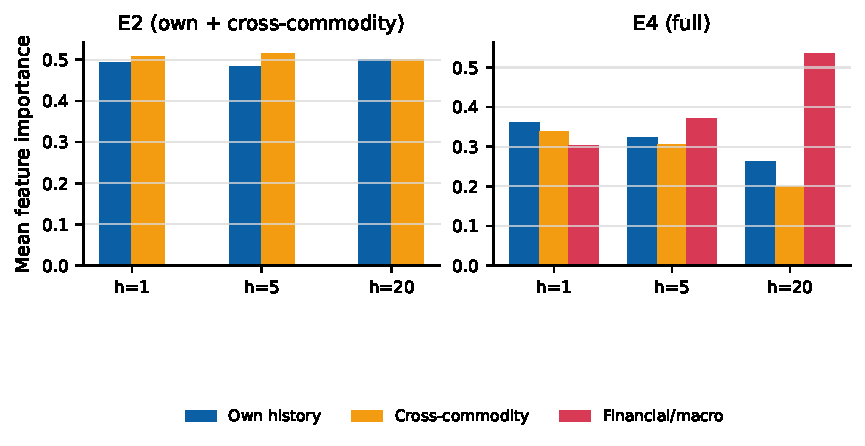
\includegraphics[width=\textwidth]{figs/fig_feature_importance.pdf}
\par\medskip
\noindent\textbf{Figure~\thefigure.} Mean feature-group importance by horizon for the E2 and E4 information sets, averaged across varieties and tree-based models.
\end{minipage}
\end{center}
\label{fig:feature_importance}

Entre os atributos individuais, \texttt{return\_lag4} e \texttt{cepea\_return} apareceram entre os mais importantes em \(h=1\) no conjunto E2. Em \(h=5\) e \(h=20\), \texttt{hist\_vol\_20} permaneceu entre os principais atributos em E2. Em E4, \texttt{selic} foi o atributo de maior importância média nos horizontes de cinco e vinte observações. Essas importâncias são diagnósticos de contribuição relativa dentro dos modelos e não representam elasticidades ou efeitos causais.

Os valores SHAP do LightGBM confirmam esse padrão e o tornam mais nítido. Com peso igual para as três séries, a participação do bloco financeiro em E4 foi de 0,386, 0,499 e 0,672 em \(h=1\), \(h=5\) e \(h=20\), enquanto o histórico próprio caiu de 0,279 para 0,190 e o bloco cross-commodity de 0,335 para 0,138. Em E2, histórico próprio e cross-commodity permaneceram equilibrados, com participação cross-commodity de 0,559, 0,504 e 0,497. Os atributos com maior SHAP médio em E4 foram \texttt{selic}, \texttt{fed\_funds} e \texttt{us\_treasury\_10y} em \(h=5\) e \(h=20\), com a Selic atingindo 0,251 em \(h=20\). Em E2, \texttt{cepea\_return} liderou em \(h=1\) e \texttt{hist\_vol\_20} em \(h=5\) e \(h=20\).

Esse resultado deve ser interpretado com cautela. As variáveis financeiras mais importantes são níveis de taxas de juros, que evoluem lentamente e acompanham tendências de longo prazo. Em modelos de árvores ajustados em janela crescente, esses níveis podem atuar como marcadores do período amostral, o que ajuda a explicar a combinação entre alta importância e ausência de ganho fora da amostra para E3 e E4 (Table~\ref{tab:ml_incremental_pooled}). De modo semelhante, a importância de \texttt{cepea\_return} pode refletir parcialmente seu padrão de ausência antes de 2016. Além disso, as importâncias nativas e SHAP são calculadas dentro da amostra descritiva completa e medem contribuição para o ajuste, não para a acurácia fora da amostra.

A Figure~\ref{fig:feature_importance} agrega arábica e conilon, o que pode ocultar diferenças específicas de variedade. A Figure~\ref{fig:variety_importance} desagrega essa mesma composição por variedade no conjunto E4. Em Arábica, a importância financeira já ultrapassa o histórico próprio e o cross-commodity em \(h=5\) e se torna dominante em \(h=20\). Em Conilon, o bloco financeiro é o menos importante em \(h=1\) e \(h=5\) e só se torna dominante em \(h=20\), enquanto a importância cross-commodity decresce de forma monótona entre os três horizontes. Como as importâncias são normalizadas para somar um em cada ajuste, a comparação entre variedades é feita apenas pela composição relativa dos blocos, e não pela magnitude absoluta. Esses resultados indicam que os fatores relevantes não são intercambiáveis entre as duas variedades.

\refstepcounter{figure}
\begin{center}
\begin{minipage}{\textwidth}
\centering
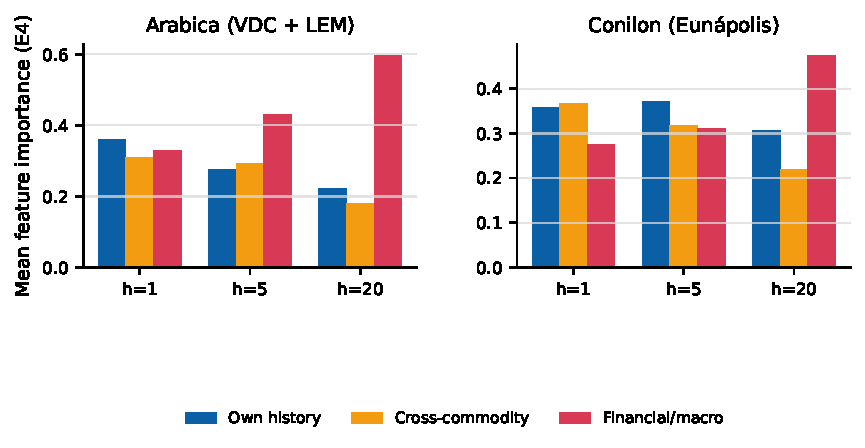
\includegraphics[width=\textwidth]{figs/fig_variety_importance.pdf}
\par\medskip
\noindent\textbf{Figure~\thefigure.} Mean feature-group importance by horizon for the E4 information set, disaggregated by coffee variety (Arabica vs.\ Conilon).
\end{minipage}
\end{center}
\label{fig:variety_importance}

\subsection{Reprodutibilidade}
\label{subsec:results_reproducibility}

O experimento foi executado em Python 3.12.10 com pandas 3.0.5, NumPy 2.5.2, arch 8.0.0, scikit-learn 1.9.0, LightGBM 4.7.0, XGBoost 3.4.1 e shap 0.52.0. A construção dos dados, os baselines, os modelos de machine learning, a validação temporal, as comparações, os testes, os regimes e a explicabilidade foram mantidos em scripts separados. O arquivo \texttt{validated\_run\_manifest.json} registra as versões, os hashes e os parâmetros principais. Os arquivos CSV de auditoria, comparação, testes, regimes e importância das variáveis preservam os resultados intermediários necessários à verificação. As análises de robustez, que incluem a sensibilidade da QLIKE, as correções para múltiplas comparações, os regimes \textit{ex ante} e a comparação entre as séries de Arábica, são executadas por um script próprio sobre as previsões fora da amostra já salvas, sem reestimação dos modelos.

\subsection{Síntese dos resultados}
\label{subsec:results_summary}

A Table~\ref{tab:rq_summary} reúne a resposta a cada pergunta de pesquisa e a evidência que a sustenta.

\begin{table*}[t]
\centering
\caption{Summary of the answers to the research questions}
\label{tab:rq_summary}
\scriptsize
\setlength{\tabcolsep}{3pt}
\begin{tabular*}{\textwidth}{@{\extracolsep{\fill}}p{3.4cm}p{2.1cm}p{7.6cm}p{2.2cm}@{}}
\hline
Pergunta & Resposta & Evidência principal & Referência \\
\hline
RQ1. ML supera os modelos econométricos? & Não & GARCH com a menor QLIKE e HAR-RV com o menor MAE e RMSE em todos os horizontes; nenhuma configuração de ML significativamente melhor que o HAR-RV em qualquer perda, nem que o GARCH em QLIKE; resultado robusto ao piso da QLIKE e à exclusão dos alvos nulos & Tables~\ref{tab:pooled_results}, \ref{tab:qlike_robust}, \ref{tab:dm_tests} \\
\hline
RQ2. Outras commodities melhoram a previsão? & Marginalmente & Ganhos pequenos e de sinal variável, restritos ao Random Forest (QLIKE +5,6\% e +2,4\% em \(h=1\) e \(h=5\)); após correção de Holm, apenas 2 comparações de MAE e 3 de erro quadrático favoráveis aos blocos ampliados & Tables~\ref{tab:rf_incremental}, \ref{tab:ml_incremental_pooled}, \ref{tab:dm_tests} \\
\hline
RQ3. Variáveis financeiras acrescentam ganho? & Não, em média & E3 e E4 pioram MAE e RMSE em todos os modelos no horizonte longo (6\% a 20\%); nenhuma melhora significativa em QLIKE & Table~\ref{tab:ml_incremental_pooled} \\
\hline
RQ4. Os resultados diferem entre regimes? & Sim, para a informação financeira & Referências econométricas superiores em todos os regimes; o bloco financeiro piora o MAE em 20\% a 27\% no regime calmo e melhora entre 1,8\% e 7,6\% no regime de alta volatilidade, diferença significativa em 6 a 7 de 9 testes HAC por modelo & Figure~\ref{fig:regime_analysis} \\
\hline
RQ5. Quais variáveis mais contribuem? & Histórico próprio e juros & Histórico próprio e cross-commodity dominam em \(h=1\) e \(h=5\); em \(h=20\), níveis de juros (Selic, Fed Funds, Treasury) concentram 67\% da participação SHAP em E4, sem ganho fora da amostra correspondente & Figures~\ref{fig:feature_importance}, \ref{fig:variety_importance} \\
\hline
RQ6. Os fatores diferem entre variedades? & Sim, na composição & Em Arábica, o bloco financeiro domina a partir de \(h=5\); em Conilon, apenas em \(h=20\), com importância cross-commodity decrescente no horizonte & Figure~\ref{fig:variety_importance} \\
\hline
\end{tabular*}
\end{table*}

Em relação a RQ1, a superioridade das referências econométricas é o resultado mais robusto do estudo. O GARCH(1,1) apresentou a menor QLIKE em todos os horizontes e em todos os cenários de robustez, e o HAR-RV apresentou o menor MAE e RMSE, com uma única exceção em Luís Eduardo Magalhães em \(h=20\). A vantagem do HAR-RV sobre todas as configurações de machine learning permaneceu significativa após as correções de Holm e Benjamini--Hochberg.

Em relação a RQ2, a informação cross-commodity foi o único bloco externo com ganhos positivos de magnitude estável, mas esses ganhos foram pequenos, restritos ao Random Forest e raramente significativos. Para o Random Forest com E2, as comparações significativamente favoráveis a 5\% foram 3 de 9 em MAE, 1 de 9 em erro quadrático e nenhuma em QLIKE. Após a correção de Holm para as 891 comparações, restaram apenas 2 comparações de MAE e 3 de erro quadrático favoráveis aos blocos ampliados em todo o desenho.

Em relação a RQ3, a informação financeira piorou a previsão em média, em todos os modelos e sobretudo no horizonte longo. Em relação a RQ4, a análise \textit{ex ante} qualifica essa conclusão: a informação financeira é prejudicial em períodos calmos, que predominam na amostra, e passa a acrescentar informação em períodos de volatilidade elevada. Esse efeito condicional não modifica a ordenação geral, pois mesmo no regime alto as referências econométricas permaneceram superiores.

Em relação a RQ5 e RQ6, os modelos atribuíram importância crescente ao bloco financeiro no horizonte longo, concentrada em níveis de juros. Como essa importância não se converteu em ganho fora da amostra, ela deve ser lida como contribuição para o ajuste dos modelos, possivelmente associada à capacidade desses níveis de marcar o período amostral, e não como evidência de valor preditivo. A composição da importância difere entre Arábica e Conilon, o que indica que os fatores associados às previsões não são intercambiáveis entre as variedades.

Em conjunto, esses resultados respondem ao objetivo do estudo. Informações de outras commodities e dos mercados financeiros não melhoram de forma sistemática a previsão da volatilidade local do café na Bahia em relação ao histórico próprio. O ganho da informação cross-commodity é marginal, e o da informação financeira é condicional ao regime de volatilidade.

\section{Discussion}
\label{sec:discussion}

Os resultados apresentados na Section~\ref{sec:experiments} mostram um quadro consistente: as referências econométricas não foram superadas, a informação cross-commodity acrescentou ganhos apenas marginais e a informação financeira piorou a previsão em média, com valor que depende do regime de volatilidade. Esta seção discute por que esse padrão emerge e o que ele significa. A Section~\ref{subsec:disc_benchmarks} examina os fatores que tornam as referências econométricas difíceis de superar nesse contexto. A Section~\ref{subsec:disc_conditional} interpreta o valor condicional da informação externa à luz da literatura de conectividade entre mercados. A Section~\ref{subsec:disc_practical} traduz os resultados em orientações para os agentes do mercado de café, e a Section~\ref{subsec:disc_limitations} apresenta as limitações do estudo.

\subsection{Por que as referências econométricas permanecem difíceis de superar}
\label{subsec:disc_benchmarks}

A principal conclusão do estudo é que modelos econométricos simples, estimados apenas com o histórico local, não foram superados por modelos de machine learning mais flexíveis nem por conjuntos de informação mais amplos. Esse resultado contrasta com estudos que reportam ganhos de modelos híbridos e de aprendizagem de máquina na previsão de volatilidade e preços agrícolas \citep{Manogna2025HybridVolatility,Zhang2025ClimateRealizedVolatility,Jin2024CoffeePriceML}, mas é consistente com revisões que mostram que os ganhos desses modelos dependem do mercado, da frequência dos dados, do horizonte e do protocolo de validação \citep{Guindani2024AgriculturalForecasting}. Três características do presente desenho ajudam a explicar a diferença.

A primeira é a natureza das séries. As cotações locais da SEAGRI-BA permanecem inalteradas em 77\% a 88\% das datas, e a volatilidade futura é nula na maior parte das origens de curto prazo. Nessas condições, a dinâmica relevante assemelha-se a uma sequência de saltos esparsos, e não a um processo contínuo com interações não lineares ricas. A vantagem de modelos flexíveis depende da existência de padrões complexos e estáveis que o histórico próprio não capture, o que é pouco provável em séries com essa densidade de informação.

A segunda é o alinhamento entre a função de estimação e a função de avaliação. O GARCH é estimado por quase-máxima verossimilhança gaussiana, cuja perda implícita coincide com a QLIKE, enquanto o HAR-RV é estimado por mínimos quadrados sobre a volatilidade e minimiza diretamente uma perda quadrática na escala avaliada. Os modelos de árvores, por sua vez, foram treinados com erro quadrático sobre a volatilidade e não incorporam a assimetria da QLIKE, que penaliza fortemente a subestimação da variância. Esse alinhamento, discutido por \citet{Patton2011VolatilityProxy} e \citet{HansenLunde2006ConsistentRanking}, explica por que cada referência vence na escala para a qual foi estimada e por que a ordenação depende da função de perda.

A terceira é a estabilidade temporal das relações. As variáveis externas mais importantes nos modelos, os níveis de juros, evoluem lentamente e acompanham tendências de longo prazo. Em árvores ajustadas em janela crescente, essas variáveis permitem particionar a amostra por período, o que melhora o ajuste dentro da amostra mas não se generaliza para anos de teste com níveis de juros fora do intervalo histórico. A combinação entre alta importância SHAP e perda fora da amostra é compatível com esse mecanismo.

\subsection{Valor condicional da informação externa}
\label{subsec:disc_conditional}

O resultado de regimes oferece uma interpretação mais precisa do papel da informação financeira. A literatura de conectividade mostra que a transmissão de volatilidade entre commodities e mercados financeiros se intensifica em crises e períodos de estresse \citep{Singh2026OilSoftCommoditySpillovers,Zhou2026CommodityConnectedness}. Os resultados deste estudo são consistentes com essa evidência em escala local: a informação financeira prejudica a previsão quando a volatilidade local é baixa e acrescenta informação quando ela é elevada. Em períodos calmos, variações de câmbio, juros ou índices acionários são interpretadas pelos modelos como sinais de risco que não se materializam nas cotações locais, o que produz previsões excessivamente voláteis. Em períodos turbulentos, a integração entre mercados aumenta e esses sinais passam a conter informação relevante.

A informação cross-commodity apresentou comportamento distinto, com ganhos pequenos e estáveis entre regimes. As variáveis desse bloco com maior importância, o indicador CEPEA e o contrato internacional de café, estão diretamente ligadas à formação do preço local. Ainda assim, mesmo duas praças da mesma variedade, sujeitas às mesmas referências de mercado, apresentam correlação de apenas 0,137 entre seus retornos e variações simultâneas de preço em apenas 5,38\% das datas comuns. Esse padrão indica que as cotações locais incorporam as referências de mercado com atraso e de forma irregular, o que limita o conteúdo preditivo contemporâneo das variáveis externas. Esse resultado é compatível com a evidência de que políticas e condições locais têm capacidade limitada de conter oscilações determinadas por forças externas, mas também de que a transmissão dessas forças aos mercados regionais não é imediata \citep{Fahmi2023LocalCoffeePolicy,AliagaMiranda2026CoffeeShocks}.

Por fim, a estabilidade do GARCH entre os períodos de estresse contrasta com a evidência de que especificações GARCH tradicionais podem apresentar limitações em períodos de instabilidade \citep{Brun2026GARCHCoffeeRisk}. No presente contexto, a vantagem do GARCH em QLIKE foi mantida antes de 2020, no choque da COVID-19, na crise de geada e oferta de 2021--2022 e no período posterior. Essa diferença pode refletir o fato de que o presente estudo avalia a previsão de variância agregada em horizontes curtos, e não medidas de risco extremo.

\subsection{Implicações práticas}
\label{subsec:disc_practical}

Para produtores, cooperativas e agentes de comercialização, os resultados sugerem uma seleção de modelos orientada pela finalidade da previsão. Quando o objetivo é dimensionar o risco em termos de variância, como no cálculo de margens ou medidas de valor em risco, o GARCH(1,1) oferece a referência mais confiável. Quando o objetivo é antecipar a magnitude típica das variações, o HAR-RV apresenta os menores erros. A inclusão de variáveis externas em modelos de machine learning não deve ser tratada como melhoria automática. Informações cross-commodity podem ser mantidas por seu custo baixo e ganho marginal, enquanto informações financeiras só se justificam em períodos de volatilidade elevada, o que sugere estratégias de combinação ou de seleção condicionadas ao regime.

\subsection{Limitações}
\label{subsec:disc_limitations}

Os resultados devem ser interpretados à luz de algumas limitações. Primeiro, as cotações locais são pouco frequentes e contêm lacunas longas, de modo que a volatilidade observada é dominada por saltos esparsos e por alvos nulos. Embora as análises de robustez mostrem que a ordenação dos modelos não depende do tratamento desses alvos, uma modelagem em duas etapas, separando a probabilidade de variação do preço e a magnitude da variação, poderia capturar melhor essa estrutura. Segundo, os modelos de machine learning foram estimados com hiperparâmetros fixos e com perda quadrática sobre a volatilidade. Essa escolha preserva a comparabilidade entre conjuntos de informação, mas não esgota o potencial desses modelos, que poderiam ser ajustados por validação temporal aninhada ou treinados com perdas alinhadas à QLIKE. Terceiro, o GARCH foi estimado com inovações normais, e distribuições com caudas pesadas podem ser mais adequadas a séries com saltos. Quarto, as variáveis financeiras de juros entraram em nível, e as importâncias nativas e SHAP foram calculadas dentro da amostra; o uso de variações e de importâncias por permutação fora da amostra permitiria separar melhor o valor preditivo do ajuste. Quinto, a junção temporal utiliza a última observação disponível até a data da cotação local, e não é possível verificar se o fechamento dos mercados externos na mesma data antecede a coleta da cotação da SEAGRI-BA. Sexto, o estudo cobre três séries de um único estado, e os contratos internacionais foram obtidos como séries contínuas do Yahoo Finance, cuja convenção de rolagem pertence à fonte. Por fim, a avaliação é estatística e não inclui medidas de valor econômico, como o desempenho de estratégias de proteção ou o teste de medidas de valor em risco.

\subsection{Síntese da discussão}

Em conjunto, a discussão indica que o desempenho inferior dos modelos de machine learning não decorre de uma falha isolada de especificação, mas da combinação entre séries locais com baixa densidade de informação, perdas de estimação desalinhadas das perdas de avaliação e variáveis externas cuja relação com a volatilidade local não é estável no tempo. Essa leitura também explica por que a informação externa não é uniformemente inútil. Seu valor aparece quando a integração entre mercados se intensifica, como nos períodos de alta volatilidade, e desaparece quando as cotações locais evoluem de forma desconectada dos mercados financeiros. A contribuição do estudo, portanto, não é apenas mostrar que modelos mais flexíveis e conjuntos de informação mais amplos não garantem previsões melhores, mas identificar em que condições e por quais mecanismos essa informação pode ser útil. As limitações apontadas definem a agenda para testar se esse padrão se mantém com modelos treinados para a perda relevante, com variáveis financeiras transformadas e com avaliações do valor econômico das previsões, questões retomadas na conclusão.

\section{Conclusion}
\label{sec:conclusion}

Este estudo avaliou se informações de outras commodities agrícolas e dos mercados financeiros melhoram a previsão fora da amostra da volatilidade futura dos preços locais de café Arábica e Conilon na Bahia. Utilizando três séries da SEAGRI-BA, quatro conjuntos de informação aninhados, modelos econométricos e de machine learning e validação temporal estrita, o estudo mostrou que a resposta é, em geral, negativa.

Os modelos econométricos estimados apenas com o histórico local permaneceram como as melhores referências: o GARCH(1,1) na escala de variância e o HAR-RV na escala de volatilidade. Esse resultado resistiu à variação do tratamento dos alvos nulos, à correção para múltiplas comparações e à decomposição por regimes e períodos de estresse. A informação cross-commodity produziu ganhos marginais e restritos ao Random Forest. A informação financeira piorou a previsão em média, mas apresentou valor condicional ao regime, prejudicando a previsão em períodos calmos e acrescentando informação em períodos de volatilidade elevada. A importância atribuída pelos modelos aos níveis de juros não se converteu em ganho fora da amostra, o que alerta para os riscos de interpretar a explicabilidade como evidência de valor preditivo.

Esses resultados indicam que, em mercados agrícolas locais com cotações pouco frequentes, a seleção de modelos deve ser orientada pela função de perda relevante para o usuário e comparada sistematicamente com referências econométricas. Pesquisas futuras podem explorar modelos em duas etapas para a ocorrência e a magnitude das variações de preço, funções de treinamento alinhadas à QLIKE, combinações de previsões condicionadas ao regime, representações da dependência dinâmica entre mercados e avaliações do valor econômico das previsões para produtores e cooperativas.

% Uncomment and use as the case may be
%\begin{theorem} 
%\end{theorem}

% Uncomment and use as the case may be
%\begin{lemma} 
%\end{lemma}

%% The Appendices part is started with the command \appendix;
%% appendix sections are then done as normal sections
%% \appendix

\section*{Disponibilidade de dados e código}
Todas as séries utilizadas são públicas: cotações locais da SEAGRI-BA, indicadores do CEPEA, séries do Banco Central do Brasil, do Federal Reserve Economic Data e da U.S. Energy Information Administration e contratos contínuos do Yahoo Finance. Os scripts de coleta, construção do painel, estimação, validação temporal, testes estatísticos, análises de robustez e figuras, bem como os arquivos de previsões fora da amostra, serão disponibilizados em \textbf{[A PREENCHER: repositório e DOI]}.

\section*{Declaração de interesses}
\textbf{[A PREENCHER pelos autores: declaração de interesses concorrentes.]}

\section*{Financiamento}
\textbf{[A PREENCHER pelos autores: agências e números de processo, ou declaração de ausência de financiamento específico.]}

\section*{Declaração de contribuição dos autores (CRediT)}
\textbf{[A PREENCHER pelos autores: papéis CRediT de cada autor, por meio do comando \texttt{\textbackslash credit\{\}} após cada \texttt{\textbackslash author}.]}

% To print the credit authorship contribution details
\printcredits

%% Loading bibliography style file
%\bibliographystyle{model1-num-names}
\bibliographystyle{cas-model2-names}

% Loading bibliography database
\bibliography{references}

% Biography
%\bio{}
% Here goes the biography details.
%\endbio

%\bio{pic1}
% Here goes the biography details.
%\endbio

\end{document}
